\documentclass[12pt,a4paper]{report}

%--------------------------------
% Packages
%--------------------------------
\usepackage[T1]{fontenc}
\usepackage[utf8]{inputenc}
\usepackage{mathptmx}
\usepackage{amsmath}
\usepackage{amssymb}
\usepackage{array}
\usepackage{tabularx}
\usepackage{longtable}
\usepackage{float}
\usepackage{graphicx}
\usepackage{grffile}
\usepackage{subcaption}
\usepackage{setspace}

% TikZ
\usepackage{tikz}
\usetikzlibrary{shapes.geometric, arrows.meta, positioning}

%--------------------------------
% Page Margins
%--------------------------------
\usepackage[
    a4paper,
    margin=1in,
    headheight=16pt
]{geometry}

%--------------------------------
% Formatting & Hyperlinks
%--------------------------------
%--------------------------------
% Table of Contents & Lists Spacing
%--------------------------------
\usepackage[titles]{tocloft}
\setlength{\cftbeforechapskip}{4pt}      % Gap before chapter entries in TOC
\setlength{\cftbeforesecskip}{1.5pt}    % Gap before section entries in TOC
\setlength{\cftbeforesubsecskip}{1pt}   % Gap before subsection entries in TOC
\setlength{\cftbeforefigskip}{3pt}      % Gap between figure entries in LOF
\setlength{\cftbeforetabskip}{3pt}      % Gap between table entries in LOT

\usepackage{titlesec}
\usepackage{fancyhdr}
\usepackage{url}
\usepackage[
    colorlinks=true,
    linkcolor=black,
    citecolor=black,
    urlcolor=blue,
    plainpages=false,
    pdfpagelabels=true
]{hyperref}

% Penalty & Tolerance (Optimized for fast compile and clean typography)
\tolerance=2000
\emergencystretch=3em
\hfuzz=2pt
\hbadness=5000
\hyphenpenalty=500
\exhyphenpenalty=500

%--------------------------------
% Paragraph Formatting
%--------------------------------
\setlength{\parindent}{0pt}
\setlength{\parskip}{6pt}

%--------------------------------
% Header & Footer
%--------------------------------
\pagestyle{fancy}
\fancyhf{}

\fancyhead[R]{Fake Review Detection Using Machine Learning}

\fancyfoot[L]{Department of Computer Applications, MACE}
\fancyfoot[R]{\thepage}

\renewcommand{\headrulewidth}{0.4pt}
\renewcommand{\footrulewidth}{0.4pt}

%--------------------------------
% Chapter Page Header & Footer
%--------------------------------
\fancypagestyle{plain}{
    \fancyhf{}

    \fancyhead[R]{Fake Review Detection Using Machine Learning}

    \fancyfoot[L]{Department of Computer Applications, MACE}
    \fancyfoot[R]{\thepage}

    \renewcommand{\headrulewidth}{0.4pt}
    \renewcommand{\footrulewidth}{0.4pt}
}

%--------------------------------
% Chapter Formatting (Preliminary Matter - Centered)
%--------------------------------
\titleformat{\chapter}[block]
{\normalfont\bfseries\fontsize{16}{20}\selectfont\centering}
{\thechapter.}
{1em}
{}

\titleformat{name=\chapter,numberless}[block]
{\normalfont\bfseries\fontsize{16}{20}\selectfont\centering}
{}
{0pt}
{}

\titlespacing*{\chapter}
{0pt}
{-30pt}
{4pt}

%--------------------------------
% Section Formatting
%--------------------------------
\titleformat{\section}
{\normalfont\bfseries\fontsize{14}{18}\selectfont\raggedright}
{\thesection}
{1em}
{}

\titlespacing*{\section}
{0pt}
{12pt}
{6pt}

%--------------------------------
% Subsection Formatting
%--------------------------------
\titleformat{\subsection}
{\normalfont\bfseries\fontsize{12}{16}\selectfont\raggedright}
{\thesubsection}
{1em}
{}

\titlespacing*{\subsection}
{0pt}
{10pt}
{4pt}

%--------------------------------
% Begin Document
%--------------------------------
\begin{document}

\onehalfspacing

% ==================================================================================================================
% FRONT PAGES (Per Mini Project Report Template)
% ==================================================================================================================

% 1. Title / Cover Page
\begin{titlepage}
\thispagestyle{empty}
\begin{center}
\vspace*{0.1cm}
{\fontsize{15}{19}\selectfont \textbf{MAR ATHANASIUS COLLEGE OF ENGINEERING}}\\[0.25em]
{\fontsize{13}{17}\selectfont \textbf{KOTHAMANGALAM}}\\[0.25em]
{\fontsize{11}{14}\selectfont \textbf{(Government Aided Autonomous Institution)}}\\[1.0cm]


\includegraphics[height=4.0cm]{figures/mace_logo.png}\\[1.0cm]

{\fontsize{14}{18}\selectfont \textbf{Department of Computer Applications}}\\[0.4em]
{\fontsize{13}{16}\selectfont Mini Project Report}\\[0.9cm]

{\fontsize{15}{21}\selectfont \textbf{FAKE REVIEW DETECTION USING MACHINE LEARNING}}\\[1.0cm]

{\fontsize{12}{15}\selectfont Done by}\\[0.4em]
{\fontsize{13}{17}\selectfont \textbf{ASHISHA S}}\\[0.2em]
{\fontsize{12}{15}\selectfont \textbf{Reg No: MAC25MCA-2017}}\\[2.5cm]

{\fontsize{12}{15}\selectfont Under the guidance of}\\[0.4em]
{\fontsize{13}{17}\selectfont \textbf{Prof.~Biju Skaria}}\\[1.0cm]

{\fontsize{12}{15}\selectfont 2025--2027}
\end{center}
\end{titlepage}

% 2. Certificate Page
\newpage
\thispagestyle{empty}
\begin{center}
\vspace*{0.1cm}
{\fontsize{13}{17}\selectfont \textbf{MAR ATHANASIUS COLLEGE OF ENGINEERING}}\\[0.2em]
{\fontsize{13}{17}\selectfont \textbf{KOTHAMANGALAM}}\\[0.2em]
{\fontsize{10.5}{13.5}\selectfont \textbf{(Government Aided Autonomous Institution)}}\\[0.6cm]


\includegraphics[height=3.5cm]{figures/mace_logo.png}\\[0.6cm]

{\fontsize{15}{19}\selectfont \textbf{CERTIFICATE}}\\[0.5cm]

{\fontsize{13}{17}\selectfont \textbf{Fake Review Detection Using Machine Learning}}\\[0.5cm]

{\fontsize{12}{18}\selectfont Certified that this is the bonafide record of project work done by}\\[0.4em]
{\fontsize{13}{17}\selectfont \textbf{ASHISHA S}}\\[0.2em]
{\fontsize{12}{16}\selectfont \textbf{Reg No: MAC25MCA-2017}}\\[0.4em]
{\fontsize{12}{18}\selectfont during the third semester, in partial fulfilment of requirements for award of the degree,}\\[0.4em]
{\fontsize{13}{17}\selectfont \textbf{Master of Computer Applications}}\\[0.3em]
{\fontsize{12}{16}\selectfont of}\\[0.3em]
{\fontsize{12}{16}\selectfont APJ Abdul Kalam Technological University, Thiruvananthapuram}\\[3cm]

\noindent
\begin{tabular}{@{}p{0.55\textwidth}r@{}}
\textbf{Prof.~Biju Skaria} & \textbf{Dr.~Sonia Abraham} \\
Faculty Guide & Head of the Department \\[1.8cm]
\textbf{Dr.~Manu John} & \textbf{Internal Examiners} \\
Project Coordinator & \\
\end{tabular}
\end{center}

% =========================================================
% 3. PRELIMINARY MATTER PAGE NUMBERING
% =========================================================

\newpage
\pagenumbering{roman}
\setcounter{page}{1}

% Roman page number centered in footer

\pagestyle{fancy}
\fancyhf{}
\fancyfoot[C]{\thepage}

\renewcommand{\headrulewidth}{0pt}
\renewcommand{\footrulewidth}{0pt}

\fancypagestyle{plain}{
    \fancyhf{}
    \fancyfoot[C]{\thepage}
    \renewcommand{\headrulewidth}{0pt}
    \renewcommand{\footrulewidth}{0pt}
}

% =========================================================
% 4. ACKNOWLEDGEMENT
% =========================================================

\chapter*{Acknowledgement}
\phantomsection
\addcontentsline{toc}{chapter}{Acknowledgement}

First and foremost, I express my gratitude to God Almighty for showering blessings and granting
the strength, perseverance, and wisdom to complete this mini-project work successfully.

I express my profound gratitude and heartfelt thanks to Dr.~Sonia Abraham, Head
of the Department of Computer Applications, Mar Athanasius College of Engineering,
Kothamangalam, for providing excellent academic facilities, lab resources, and continuous
encouragement throughout this endeavour.

I extend my deep gratitude and sincere appreciation to my project guide, Prof.~Biju Skaria, for
invaluable guidance, constructive suggestions, insightful feedback, and patient support rendered
during all stages of this project development.

I am also thankful to the Project Coordinator, faculty members, and technical staff of the
Department of Computer Applications for their kind cooperation, guidance, and assistance.
Finally, I express my deepest appreciation to my parents, family members, and friends for their
continuous moral support, understanding, and encouragement throughout the completion of this
project.


\vspace{1.5cm}

\begin{flushright}
\text{Ashisha S}\\
\text{MAC25MCA-2017}\\
\end{flushright}

% =========================================================
% 5. ABSTRACT
% =========================================================

\newpage

\chapter*{Abstract}
\phantomsection
\addcontentsline{toc}{chapter}{Abstract}

Online reviews play an important role in influencing
consumer decisions and establishing trust in digital
platforms. However, the increasing presence of fake
and deceptive reviews creates challenges for users
in identifying reliable information. This project,
Fake Review Detection Using Machine Learning,
focuses on developing a machine learning-based
system capable of classifying hotel reviews as
Fake/Deceptive or Genuine/Truthful based on
their textual characteristics.

The system is developed using the Ott et al.
Gold Standard Deceptive Opinion Spam dataset,
which contains 1,600 labelled hotel reviews.
The dataset undergoes exploratory data analysis,
text preprocessing, and feature extraction.
Term Frequency-Inverse Document Frequency
(TF-IDF) is used to represent textual information,
while linguistic features and VADER sentiment
scores are investigated as additional features
for review classification.

Three supervised machine learning algorithms,
namely Logistic Regression, Linear Support Vector
Machine, and Random Forest, are evaluated using
different feature combinations. The models are
compared using classification performance measures
to identify a suitable configuration for fake
review detection.

The experimental results show that Logistic
Regression with TF-IDF and VADER sentiment
features provides the best overall classification
performance, achieving an accuracy of 91.88\%
on the original test dataset. The selected model
is further evaluated using a balanced external
dataset of 500 unseen reviews (250 fake and
250 genuine), of which 452 are correctly classified.

A Streamlit-based web application is developed
to provide an interactive interface where users
can enter hotel reviews and obtain predictions
along with class probabilities and explanations
of the classification process. The proposed
system demonstrates the practical application
of machine learning and Natural Language
Processing techniques for identifying
potentially deceptive online reviews.

% =========================================================
% 6. LIST OF TABLES
% =========================================================

\newpage
\phantomsection
\addcontentsline{toc}{chapter}{List of Tables}
\listoftables

% =========================================================
% 7. LIST OF FIGURES
% =========================================================

\newpage
\phantomsection
\addcontentsline{toc}{chapter}{List of Figures}
\listoffigures

% =========================================================
% 8. TABLE OF CONTENTS
% =========================================================

\newpage
\pagestyle{empty}
\addtocontents{toc}{\protect\thispagestyle{empty}}
\renewcommand{\contentsname}{Contents}
\tableofcontents

% =========================================================
% MAIN BODY
% Arabic Page Numbering and Running Headers / Footers
% =========================================================

\newpage
\pagenumbering{arabic}
\setcounter{page}{1}

\pagestyle{fancy}
\fancyhf{}

\fancyhead[R]{Fake Review Detection Using Machine Learning}

\fancyfoot[L]{Department of Computer Applications, MACE}
\fancyfoot[R]{\thepage}

\renewcommand{\headrulewidth}{0.4pt}
\renewcommand{\footrulewidth}{0.4pt}

\fancypagestyle{plain}{
    \fancyhf{}

    \fancyhead[R]{Fake Review Detection Using Machine Learning}

    \fancyfoot[L]{Department of Computer Applications, MACE}
    \fancyfoot[R]{\thepage}

    \renewcommand{\headrulewidth}{0.4pt}
    \renewcommand{\footrulewidth}{0.4pt}
}

%--------------------------------
% Chapter Formatting (Left-Aligned from Introduction onwards)
%--------------------------------
\titleformat{\chapter}[block]
{\normalfont\bfseries\fontsize{16}{20}\selectfont\raggedright}
{\thechapter.}
{1em}
{}

\titleformat{name=\chapter,numberless}[block]
{\normalfont\bfseries\fontsize{16}{20}\selectfont\raggedright}
{}
{0pt}
{}

%================================
% CHAPTER 1
%================================
\chapter{Introduction}

Online reviews have become an important source of information
for consumers when making decisions about products and services.
Customers rely on these reviews to evaluate quality, reliability,
and overall experiences. However, the growing popularity of
online review platforms has also increased the presence of
fake or deceptive reviews. Such reviews may be written to
promote a business, damage competitors' reputations, or
mislead potential customers. This reduces the credibility
of online platforms and makes it difficult to distinguish
genuine opinions from misleading information.

Machine Learning (ML) and Natural Language Processing (NLP)
techniques provide an approach for automatically detecting
deceptive reviews. Machine learning algorithms learn patterns
from labelled data to classify reviews as fake or genuine,
while NLP techniques process and analyse textual information.
Feature extraction methods convert review content into
numerical representations by considering textual, linguistic,
and sentiment-based characteristics.

This project uses the Ott Deceptive Opinion Spam Corpus,
a gold-standard dataset containing 1,600 labelled hotel
reviews, including 800 deceptive and 800 truthful reviews.
The review text undergoes preprocessing techniques such as
lowercase conversion, removal of unnecessary characters,
tokenization, stop-word removal, and lemmatization.
Term Frequency-Inverse Document Frequency (TF-IDF)
is used for textual representation. Additional linguistic
features, including review length, sentence count, and
punctuation-related characteristics, are extracted.
VADER sentiment analysis is also applied to obtain
positive, negative, neutral, and compound sentiment scores.

Three supervised machine learning algorithms, namely
Logistic Regression, Linear Support Vector Machine (SVM),
and Random Forest, are considered for classification.
Different combinations of textual, linguistic, and
sentiment-based features are examined. The models are
evaluated using Accuracy, Precision, Recall, F1-score,
ROC--AUC, and Confusion Matrix to compare their
classification performance.

The main objective of this project is to develop a
machine learning-based system capable of identifying
fake and genuine hotel reviews. By integrating NLP,
feature extraction, sentiment analysis, and supervised
machine learning techniques, the system aims to provide
a practical approach for detecting deceptive reviews
and improving the reliability of online review platforms.

%================================
% CHAPTER 2
%================================
\newpage
\chapter{Supporting Literature}

\section{Literature Review}

%--------------------------------
% PAPER I
%--------------------------------

\textbf{Paper I}

\textit{A. Khan, M. Adnan, and S. Anwar (2025). Empowering Trust in Digital Platforms: Sentiment Analysis and Emotion AI for Fake Reviews Detection. IEEE Transactions on Computational Social Systems, Early Access. doi:10.1109/TCSS.2025.3638615.}

Khan et al. (2025) investigated the use of sentiment analysis and linguistic characteristics for detecting fake online reviews. The study highlights that fake and genuine reviews can exhibit different linguistic and emotional patterns. Therefore, sentiment information can be used together with textual and linguistic features to provide additional information for fake review classification.

The study used three publicly available review datasets from different domains, including Android application reviews, hotel reviews, and product reviews. The datasets contain reviews from different application areas, allowing the proposed approach to be evaluated across multiple domains. The study investigated linguistic characteristics such as review length, punctuation, misspellings, adjective usage, and textual similarity along with sentiment-related information.

The methodology includes data preprocessing, linguistic feature extraction, sentiment analysis, machine learning classification, feature importance analysis, and performance evaluation. TF-IDF was used to represent textual information, while sentiment and emotion-related characteristics were extracted to provide additional information about the reviews. Feature analysis was also performed to identify important characteristics contributing to classification.

The study used Random Forest and Decision Tree classifiers for fake review detection. Information gain and approximation-based feature analysis were used for feature selection and analysis, while SHAP was used to interpret the contribution of individual features to the model predictions.

The results demonstrated that integrating linguistic features with sentiment analysis can improve fake review detection performance. The study reported high classification performance for the evaluated datasets, with Random Forest and Decision Tree achieving accuracy of up to approximately 98\% with high F1-scores. The findings indicate that sentiment and linguistic characteristics can complement conventional textual information and provide useful signals for identifying deceptive reviews.

The study also highlights the importance of understanding the contribution of individual features to fake review classification. However, the proposed project uses a smaller and more practical feature set that can be directly extracted from the available review text. The proposed system combines TF-IDF features with linguistic and VADER sentiment features using the Ott Deceptive Opinion Spam Corpus.

\begin{table}[H]
\centering
\small
\renewcommand{\arraystretch}{1.3}

\begin{tabularx}{0.95\textwidth}{|>{\raggedright\arraybackslash}p{0.27\textwidth}|X|}
\hline
\textbf{Title} &
Empowering Trust in Digital Platforms: Sentiment Analysis and Emotion AI for Fake Reviews Detection \\
\hline

\textbf{Authors} &
A. Khan, M. Adnan, and S. Anwar \\
\hline

\textbf{Year} &
2025 \\
\hline

\textbf{Area of Work} &
Fake review detection using linguistic characteristics, sentiment analysis, feature analysis, and machine learning. \\
\hline

\textbf{Dataset Used} &
Three publicly available datasets consisting of Android application reviews, hotel reviews, and product reviews. \\
\hline

\textbf{Methodology} &
Data preprocessing, TF-IDF feature extraction, linguistic feature extraction, sentiment and emotion analysis, feature analysis, machine learning classification, SHAP-based interpretation, and performance evaluation. \\
\hline

\textbf{Algorithms Used} &
Random Forest and Decision Tree. \\
\hline

\textbf{Key Findings} &
The study demonstrated that combining linguistic features with sentiment information can improve fake review detection. The evaluated models achieved high classification performance, with accuracy of up to approximately 98\% and high F1-scores. \\
\hline

\end{tabularx}

\caption{Summary of Paper I}
\label{tab:paper1}
\end{table}

%--------------------------------
% PAPER II
%--------------------------------

\newpage

\textbf{Paper II}

\textit{M. Abdulqader, A. Namoun, and Y. Alsaawy (2022). Fake Online Reviews: A Unified Detection Model Using Deception Theories. IEEE Access, Vol. 10, pp. 128622--128655. doi:10.1109/ACCESS.2022.3227631.}

Abdulqader et al. (2022) proposed a unified framework for detecting fake online reviews by combining deception theories with machine learning techniques. The study focuses on identifying characteristics that can distinguish deceptive reviews from truthful reviews. Instead of relying only on conventional textual features, the authors used deception theories to identify both verbal and non-verbal characteristics related to fake reviews.

The proposed methodology consists of several stages, including the selection of deception theories, identification of measurable deception constructs, feature extraction, machine learning-based classification, and experimental evaluation. The authors identified nine important deception constructs, including specificity, quantity, non-immediacy, affect, uncertainty, informality, consistency, source credibility, and deviation in behaviour. These constructs were represented using verbal and non-verbal features obtained from review content and reviewer-related information.

For experimental evaluation, the study used three Yelp benchmark datasets, namely YelpChi, YelpNYC, and YelpZip. The review data were processed and relevant features were extracted before applying machine learning algorithms. Logistic Regression, Naive Bayes, Decision Tree, and Random Forest were evaluated for fake review classification.

The results showed that deception-related constructs were useful for identifying fake reviews. The study found that non-verbal features were important for distinguishing fake reviews and that combining verbal and non-verbal features improved detection performance. The theory-based approach also provided useful interpretability with relatively low computational complexity.

An important limitation of this approach is its dependence on reviewer behavioural and metadata information, which may not always be available in practical review detection systems. This motivates the proposed project to focus mainly on information that can be obtained directly from review content.

Based on these findings, the proposed system focuses on review text and uses textual, linguistic, and sentiment-based features. The proposed project uses the Ott Deceptive Opinion Spam Corpus rather than the Yelp benchmark datasets used in this study.

\begin{table}[H]
\centering
\small
\renewcommand{\arraystretch}{1.3}

\begin{tabularx}{0.95\textwidth}{|>{\raggedright\arraybackslash}p{0.27\textwidth}|X|}
\hline
\textbf{Title} &
Fake Online Reviews: A Unified Detection Model Using Deception Theories \\
\hline

\textbf{Authors} &
M. Abdulqader, A. Namoun, and Y. Alsaawy \\
\hline

\textbf{Year} &
2022 \\
\hline

\textbf{Area of Work} &
Theory-driven fake review detection using verbal and non-verbal deception features combined with machine learning. \\
\hline

\textbf{Dataset Used} &
YelpChi, YelpNYC, and YelpZip benchmark datasets. \\
\hline

\textbf{Methodology} &
Selection of deception theories, deception construct identification, verbal and non-verbal feature extraction, machine learning classification, and experimental evaluation. \\
\hline

\textbf{Algorithms Used} &
Logistic Regression, Naive Bayes, Decision Tree, and Random Forest. \\
\hline

\textbf{Key Findings} &
Deception-related features were useful for identifying fake reviews. Non-verbal features were important, and combining verbal and non-verbal features improved fake review detection performance. \\
\hline

\end{tabularx}

\caption{Summary of Paper II}
\label{tab:paper2}
\end{table}

%--------------------------------
% PAPER III
%--------------------------------

\newpage

\textbf{Paper III}

\textit{S. Janokar, K. Joshi, K. More, P. Pawar, R. Raikwar, and T. Singh (2024). Fake Review Detection System: A Machine Learning Approach with Linguistic and Semantic Analysis. Proceedings of the 2024 International Conference on Artificial Intelligence and Quantum Computation-Based Sensor Application (ICAIQSA). doi:10.1109/ICAIQSA64000.2024.10882276.}

Janokar et al. (2024) proposed a machine learning-based Fake Review Detection System that incorporates linguistic and semantic analysis for identifying fake reviews. The study emphasizes that fake review detection should consider not only the textual characteristics of reviews but also non-linguistic behavioural characteristics of reviewers.

The study used review data containing authentic and counterfeit reviews obtained from an online review platform. Yelp review data were considered in the study because Yelp's review filtering system provides categorized review information that can be used for fake review detection research. The data were preprocessed through text normalization and removal of irrelevant characters. Techniques were also applied to handle class imbalance and provide a more balanced representation of genuine and fake reviews.

Natural Language Processing techniques were used to extract linguistic and semantic features from the review text. TF-IDF and word embeddings were used to represent textual and semantic information. The study also developed custom linguistic and semantic analysis components to capture subtle characteristics that may indicate deceptive reviews.

Several classical machine learning algorithms were examined, including Random Forest, Support Vector Machine, Decision Tree, and Logistic Regression. Hyperparameters were adjusted to improve classification performance, and cross-validation was used to evaluate model robustness and reduce the possibility of overfitting.

The study evaluated the detection system using Accuracy, Precision, Recall, F1-score, AUC, and Confusion Matrix. The reported model achieved approximately 99.97\% accuracy, 99.94\% F1-score, 99.97\% recall, and 99.97\% AUC. The confusion matrix also showed a high number of correct predictions with comparatively fewer incorrect predictions.

The study further examined the relationship between user behavioural features, textual features, and model confidence. The authors reported that non-linguistic behavioural characteristics were important for fake review detection and that combining behavioural and textual information could improve the effectiveness of the detection system.

The findings of this study provide motivation for the proposed project to use linguistic and semantic information for fake review detection. However, the proposed project focuses specifically on review text and does not depend on reviewer behavioural information. TF-IDF features are combined with six linguistic features and four VADER sentiment features to represent the reviews. Logistic Regression, Linear SVM, and Random Forest will be used for classification. The models will be evaluated using Accuracy, Precision, Recall, F1-score, ROC--AUC, and Confusion Matrix.

\begin{table}[H]
\centering
\small
\renewcommand{\arraystretch}{1.4}

\begin{tabularx}{0.95\textwidth}{|>{\raggedright\arraybackslash}p{0.27\textwidth}|X|}
\hline
\textbf{Title} &
Fake Review Detection System: A Machine Learning Approach with Linguistic and Semantic Analysis \\
\hline

\textbf{Authors} &
S. Janokar, K. Joshi, K. More, P. Pawar, R. Raikwar, and T. Singh \\
\hline

\textbf{Year} &
2024 \\
\hline

\textbf{Area of Work} &
Machine learning-based fake review detection using linguistic, semantic, and non-linguistic behavioural features. \\
\hline

\textbf{Dataset Used} &
Online review data containing authentic and counterfeit reviews, with Yelp review data considered for fake review detection. \\
\hline

\textbf{Methodology} &
Data preprocessing, handling of imbalanced data, linguistic and semantic feature extraction, TF-IDF, word embeddings, machine learning classification, hyperparameter adjustment, cross-validation, and performance evaluation. \\
\hline

\textbf{Algorithms Used} &
Random Forest, Support Vector Machine, Decision Tree, and Logistic Regression. \\
\hline

\textbf{Key Findings} &
The study reported that combining textual and non-linguistic behavioural characteristics can improve fake review detection. The reported model achieved approximately 99.97\% accuracy, 99.94\% F1-score, 99.97\% recall, and 99.97\% AUC. \\
\hline

\end{tabularx}

\caption{Summary of Paper III}
\label{tab:paper3}
\end{table}

\newpage

\section{Literature Review Summary}

The reviewed literature demonstrates that machine learning
and Natural Language Processing techniques can be effectively
used for detecting deceptive online reviews. The studies
explore different combinations of textual, linguistic,
sentiment-based, semantic, and behavioural features to
distinguish fake reviews from genuine reviews. The literature
also shows that combining multiple feature types can provide
useful information for classification beyond textual
information alone.

Table \ref{tab:litsummary} presents a summary of the
reviewed research papers, highlighting their methodologies
and major contributions.

\begin{longtable}{|
>{\raggedright\arraybackslash}p{0.30\textwidth}|
>{\raggedright\arraybackslash}p{0.62\textwidth}|}
\hline

\textbf{Paper Title} &
\textbf{Summary} \\
\hline
\endfirsthead

\hline
\textbf{Paper Title} &
\textbf{Summary} \\
\hline
\endhead

\textbf{Paper I}

Empowering Trust in Digital Platforms:
Sentiment Analysis and Emotion AI for
Fake Reviews Detection
&
The study investigates fake review detection using
Android application, hotel, and product review datasets.
It examines linguistic characteristics such as review
length, punctuation, misspellings, adjective usage,
and textual similarity, along with sentiment and
emotion-related features.

Random Forest and Decision Tree algorithms are used
for classification. The study highlights the usefulness
of combining linguistic and sentiment information
and employs SHAP to interpret the contribution of
individual features to model predictions.
\\
\hline

\textbf{Paper II}

Fake Online Reviews: A Unified Detection
Model Using Deception Theories
&
The research introduces a theory-driven approach
to fake review detection using the YelpChi,
YelpNYC, and YelpZip datasets. It combines
verbal deception features derived from review
text with non-verbal features associated with
reviewer behaviour.

Logistic Regression, Naive Bayes, Decision Tree,
and Random Forest algorithms are evaluated.
The study demonstrates the importance of
combining verbal and non-verbal deception
indicators for improving fake review detection.
\\
\hline

\textbf{Paper III}

Fake Review Detection System:
A Machine Learning Approach with
Linguistic and Semantic Analysis
&
The study proposes a machine learning-based
fake review detection system using Yelp
review data. It incorporates linguistic and
semantic information through TF-IDF,
word embeddings, and non-linguistic
behavioural characteristics.

Random Forest, Support Vector Machine,
Decision Tree, and Logistic Regression
algorithms are used for classification.
The research demonstrates the effectiveness
of combining linguistic, semantic, and
behavioural features using classical
machine learning techniques.
\\
\hline

\caption{Summary of Reviewed Literature}
\label{tab:litsummary}\\
\end{longtable}

\section{Findings and Proposals}

The literature review highlights several important findings
that guide the development of the proposed Fake Review
Detection System. The major findings are summarized below:

\begin{enumerate}

\item \textbf{Feature Combination:}
The reviewed studies indicate that combining different
types of features can improve fake review detection.
Textual, linguistic, sentiment-based, semantic, and
behavioural characteristics capture different aspects
of review content. Therefore, the proposed system will
examine different combinations of TF-IDF, linguistic,
and sentiment-based features to determine their
effectiveness in classification.

\item \textbf{Linguistic Features:}
Previous studies suggest that linguistic characteristics,
such as review length, word usage, and punctuation,
can provide useful information for identifying deceptive
reviews. The proposed system will investigate six
linguistic features: Review Length, Sentence Count,
Average Word Length, Exclamation Count, Question Count,
and Capital Count.

\item \textbf{Sentiment Analysis:}
Sentiment-related characteristics can provide additional
information about the emotional patterns expressed in
reviews. Therefore, VADER sentiment analysis will be
used to extract four sentiment features: Positive,
Negative, Neutral, and Compound scores.

\item \textbf{Classical Machine Learning:}
The reviewed studies demonstrate the effectiveness
of classical machine learning algorithms for fake
review classification. Therefore, Logistic Regression,
Linear Support Vector Machine (SVM), and Random Forest
will be considered for the proposed system.

\item \textbf{Practical Feature Selection:}
Some existing approaches depend on reviewer behavioural
information or metadata, which may not always be
available. Therefore, the proposed system will focus
on features that can be extracted directly from
review text.

\end{enumerate}

Based on these findings, this project proposes a
machine learning-based Fake Review Detection System
using the Ott Deceptive Opinion Spam Corpus.
The review text will undergo NLP preprocessing,
including HTML tag removal, lowercase conversion,
removal of URLs, numbers, punctuation and special
characters, tokenization, stop-word removal,
and lemmatization.

TF-IDF with unigram and bigram features will be
used for textual representation. Six linguistic
features and four VADER sentiment features will
also be extracted to analyse writing characteristics
and sentiment information. Four feature configurations
will be considered: TF-IDF alone, TF-IDF with
linguistic features, TF-IDF with VADER sentiment
features, and TF-IDF with both linguistic and
VADER features.

These feature configurations will be evaluated
using Logistic Regression, Linear SVM, and Random
Forest classifiers. Model performance will be
compared using Accuracy, Precision, Recall,
F1-score, ROC--AUC, and Confusion Matrix to
identify a suitable classification approach
for the proposed system.

\newpage
\chapter{System Analysis}

System analysis defines the framework of the proposed Fake Review Detection System by studying the dataset, identifying its important characteristics, and determining the preprocessing, feature extraction, and machine learning techniques required for fake review classification. This chapter presents the analysis of the Ott gold-standard dataset and describes the proposed preprocessing and feature extraction approach.

\section{Analysis of Dataset}

\subsection{About the Dataset}

The proposed Fake Review Detection System uses the Ott Deceptive Opinion Spam Corpus, a gold-standard dataset developed for the study of deceptive online reviews. The dataset contains labelled hotel reviews and is used for binary classification of deceptive and truthful reviews. The review text will be the primary source of information for Natural Language Processing (NLP), while the rating and class label will be considered during data analysis and feature extraction.

The dataset contains 1600 hotel reviews and three relevant attributes: \texttt{Ori\_Review}, \texttt{Rating}, and \texttt{Label}. The \texttt{Label} attribute is the target variable, representing the two classes of reviews. The dataset consists of 800 deceptive reviews and 800 truthful reviews, resulting in an equal distribution between the two classes.

The dataset contains textual and numerical attributes. The review text stored in \texttt{Ori\_Review} will be processed using NLP techniques and represented using TF-IDF. Additional features such as review length, sentence count, average word length, and sentiment scores will also be considered to capture different characteristics of the reviews. VADER sentiment analysis will be used to extract positive, negative, neutral, and compound sentiment features.

The dataset contains an equal number of deceptive and truthful reviews, making it suitable for binary classification without requiring additional class balancing techniques. The extracted features will be combined and used to train Logistic Regression, Linear Support Vector Machine (SVM), and Random Forest classification models.

\begin{table}[H]
\centering
\small
\renewcommand{\arraystretch}{1.3}
\begin{tabularx}{0.95\textwidth}{|>{\raggedright\arraybackslash}p{0.30\textwidth}|X|}
\hline
\textbf{Property} & \textbf{Description} \\
\hline
Dataset Name & Ott Deceptive Opinion Spam Corpus \\
\hline
Total Reviews & 1600 \\
\hline
Number of Attributes & 3 \\
\hline
Problem Type & Binary Classification \\
\hline
Target Variable & \texttt{Label} \\
\hline
Target Classes & Deceptive (Fake), Truthful (Genuine) \\
\hline
Data Types & Numerical and Textual \\
\hline
Primary Feature & \texttt{Ori\_Review} (Hotel Review Text) \\
\hline
\end{tabularx}
\caption{Characteristics of the Dataset}
\label{tab:datasetdescription}
\end{table}

\begin{table}[H]
\centering
\small
\renewcommand{\arraystretch}{1.3}
\begin{tabularx}{0.95\textwidth}{|>{\raggedright\arraybackslash}p{0.30\textwidth}|X|}
\hline
\textbf{Attribute} & \textbf{Description} \\
\hline
\texttt{Ori\_Review} & Hotel review text used as the primary input for NLP and TF-IDF feature extraction. \\
\hline
\texttt{Rating} & Numerical rating associated with the hotel review. \\
\hline
\texttt{Label} & Target class indicating whether the review is deceptive or truthful. \\
\hline
\end{tabularx}
\caption{Description of Dataset Attributes}
\label{tab:datasetattributes}
\end{table}

The dataset is particularly suitable for the proposed system because it provides manually labelled deceptive and truthful hotel reviews, allowing supervised machine learning algorithms to learn patterns associated with deceptive review writing. The balanced distribution of the two classes also allows the performance of the classification models to be compared using multiple evaluation measures without the results being dominated by one class.

\subsection{Explore the Dataset}

Exploratory Data Analysis (EDA) was performed to understand the structure, quality, and characteristics of the Ott gold-standard dataset before model development. Basic operations such as \texttt{shape}, \texttt{info()}, \texttt{dtypes}, \texttt{describe()}, missing value analysis, duplicate detection, and class distribution analysis were used to examine the dataset.

The dataset contains 1600 hotel reviews with four attributes. The \texttt{Ori\_Review} attribute contains the original review text and serves as the primary source of information for classification. The \texttt{Rating} attribute provides the numerical rating associated with each review, while the \texttt{Label} attribute represents the target class. The \texttt{Unnamed: 0} attribute is an index column and is not used as a feature during model training.

The class distribution was examined to determine whether the dataset required any balancing technique. The dataset contains 800 deceptive reviews and 800 truthful reviews, resulting in an equal distribution between the two classes. Therefore, no additional class balancing technique was required. The results of the exploratory analysis were used to guide the subsequent preprocessing and feature extraction stages.

\begin{figure}[H]
    \centering
    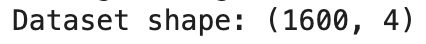
\includegraphics[
        width=0.28\textwidth,
        height=0.25\textheight,
        keepaspectratio
    ]{figures/shape.png}
    \caption{Shape of the Dataset}
    \label{fig:shape}
\end{figure}

\begin{figure}[H]
    \centering
    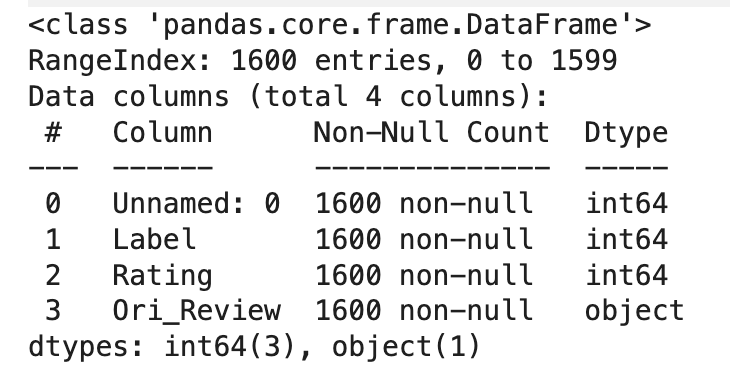
\includegraphics[
        width=0.50\textwidth,
        height=0.40\textheight,
        keepaspectratio
    ]{figures/info.png}
    \caption{Dataset Information}
    \label{fig:info}
\end{figure}

\begin{figure}[H]
    \centering
    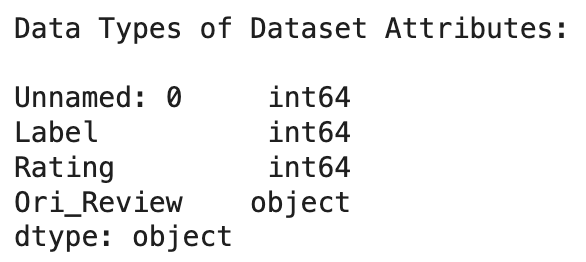
\includegraphics[
        width=0.40\textwidth,
        height=0.30\textheight,
        keepaspectratio
    ]{figures/dtypes.png}
    \caption{Data Types of Dataset Attributes}
    \label{fig:dtypes}
\end{figure}

\begin{figure}[H]
    \centering
    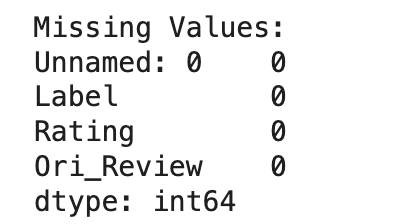
\includegraphics[
        width=0.30\textwidth,
        height=0.30\textheight,
        keepaspectratio
    ]{figures/missing_values.png}
    \caption{Missing Value Analysis}
    \label{fig:missing}
\end{figure}

\begin{figure}[H]
    \centering
    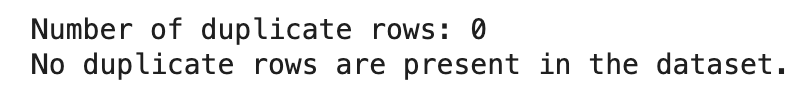
\includegraphics[
        width=0.45\textwidth,
        height=0.20\textheight,
        keepaspectratio
    ]{figures/duplicate.png}
    \caption{Duplicate Record Analysis}
    \label{fig:duplicate}
\end{figure}

\begin{figure}[H]
    \centering
    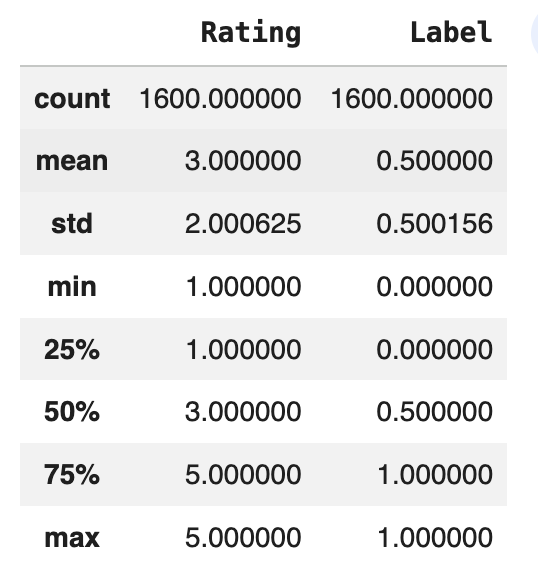
\includegraphics[
        width=0.30\textwidth,
        height=0.30\textheight,
        keepaspectratio
    ]{figures/describe.png}
    \caption{Statistical Summary of Numerical Attributes}
    \label{fig:describe}
\end{figure}

\begin{figure}[H]
    \centering
    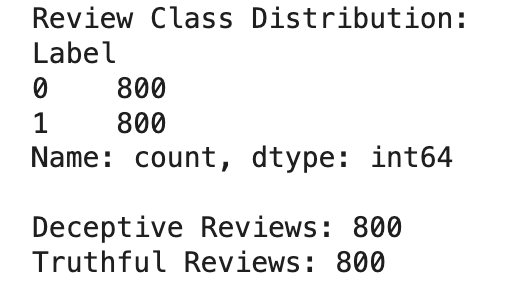
\includegraphics[
        width=0.40\textwidth,
        height=0.40\textheight,
        keepaspectratio
    ]{figures/class_distribution1.png}
    \caption{Class Count Summary of Review Labels}
    \label{fig:class_distribution1}
\end{figure}

\section{Data Preprocessing}

Data preprocessing is an important stage in the development of a machine learning model because the quality of the input data can affect the performance of the classification model. Online reviews may contain HTML tags, different text formats, punctuation, common words, and other textual variations. Therefore, the review text needs to be cleaned and converted into a suitable format before feature extraction and model training.

In the proposed Fake Review Detection System, the preprocessing stage mainly consists of data cleaning, feature engineering, and text feature representation. The review text is first cleaned using Natural Language Processing (NLP) techniques. After cleaning, selected linguistic and sentiment-based features are extracted from the reviews. The textual information is then represented numerically using Term Frequency-Inverse Document Frequency (TF-IDF). These features are combined and selected as inputs for the machine learning models.

\subsection{Data Cleaning}

Data cleaning is the first stage of preprocessing and is performed to remove unnecessary variations from the review text. The objective is to obtain a consistent representation of the reviews while retaining the meaningful textual information required for classification.

In the proposed system, the review text stored in the \texttt{Ori\_Review} attribute is processed through a sequence of NLP operations. The implemented cleaning steps include HTML tag removal, lowercase conversion, removal of punctuation and special characters, tokenization, stop-word removal, and lemmatization. The resulting cleaned text is then used for subsequent feature extraction and TF-IDF vectorization.

\subsubsection*{HTML Tag Removal}

HTML tags present in the review text are removed to eliminate unnecessary markup and retain only the actual textual content of the review. This step helps ensure that HTML elements do not become part of the textual features used during classification.

\subsubsection*{Lowercase Conversion}

All review text is converted into lowercase to maintain consistency in the text data. This prevents words with different letter cases, such as ``Excellent'' and ``excellent'', from being treated as different terms during feature extraction.

\subsubsection*{Removal of Punctuation and Special Characters}

Punctuation marks and special characters are removed from the review text to reduce unnecessary textual variations. This produces a simpler representation of the review text for subsequent NLP operations.

\subsubsection*{Tokenization}

Tokenization divides the cleaned review text into individual words or tokens. This allows the text to be processed at the word level during subsequent preprocessing operations.

\subsubsection*{Stop-word Removal}

Commonly occurring words that provide limited useful information for classification are removed from the tokenized reviews. Examples include words such as ``the'', ``is'', ``and'', and ``of''. Removing these words helps reduce unnecessary terms before feature extraction.

\subsubsection*{Lemmatization}

Lemmatization converts words into their base or dictionary form. It helps reduce different forms of the same word and provides a more consistent representation of the review text. The lemmatized tokens are then combined to obtain the final cleaned review text.


\subsection{Analysis of Feature Variables}

After text preprocessing, feature extraction was performed to convert the processed reviews into numerical representations suitable for machine learning. The feature set consists of TF-IDF features, linguistic features, and sentiment-based features extracted using VADER.

\subsubsection*{TF-IDF Features}

Term Frequency-Inverse Document Frequency (TF-IDF) was used to represent the textual content of the reviews numerically. Both unigram and bigram features were extracted to capture individual words as well as meaningful two-word combinations. The TF-IDF representation was configured with a maximum of 10,000 features, a minimum document frequency of 2, and a maximum document frequency of 0.95. Sublinear term frequency scaling was also applied to reduce the influence of very frequent terms.

\subsubsection*{Linguistic Features}

Additional linguistic features were extracted from the review text to capture structural and stylistic characteristics of the reviews. The following six linguistic features were used:

\begin{itemize}
    \item \textbf{Review Length:} Represents the total length of a review in terms of words.
    
    \item \textbf{Sentence Count:} Represents the number of sentences contained in the review.
    
    \item \textbf{Average Word Length:} Represents the average number of characters per word in the review.
    
    \item \textbf{Exclamation Count:} Represents the number of exclamation marks present in the review.
    
    \item \textbf{Question Count:} Represents the number of question marks present in the review.
    
    \item \textbf{Capital Count:} Represents the number of uppercase characters present in the review.
\end{itemize}

These features help capture differences in writing style and structural patterns between fake and genuine reviews.

\subsubsection*{VADER Sentiment Features}

VADER (Valence Aware Dictionary and sEntiment Reasoner) was used to extract sentiment-related characteristics from the reviews. Four sentiment features were obtained:

\begin{itemize}
    \item \textbf{Positive:} Represents the proportion of text associated with positive sentiment.
    
    \item \textbf{Negative:} Represents the proportion of text associated with negative sentiment.
    
    \item \textbf{Neutral:} Represents the proportion of text associated with neutral sentiment.
    
    \item \textbf{Compound:} Represents the overall normalized sentiment score of the review, ranging from -1 to +1.
\end{itemize}

The TF-IDF, linguistic, and VADER sentiment features are combined to form the final feature representation used for the proposed classification models.

\subsection{Analysis of Class Variables}

The target variable of the Ott Deceptive Opinion Spam Corpus is the \texttt{Label} attribute, which represents the class of each review. The problem is formulated as a binary classification task in which each review belongs to either the fake or genuine class.

The class labels used in the dataset are defined as follows:

\begin{itemize}
    \item Fake / Deceptive Review (Label = 1)
    \item Genuine / Truthful Review (Label = 0)
\end{itemize}

The dataset contains an equal number of fake and genuine reviews. There are 800 reviews labelled as fake or deceptive and 800 reviews labelled as genuine or truthful, giving a total of 1600 reviews. Therefore, each class represents 50\% of the dataset.

\begin{table}[H]
\centering
\renewcommand{\arraystretch}{1.3}
\begin{tabular}{|c|c|c|}
\hline
\textbf{Class} & \textbf{Number of Reviews} & \textbf{Percentage} \\
\hline
Fake / Deceptive Reviews & 800 & 50\% \\
\hline
Genuine / Truthful Reviews & 800 & 50\% \\
\hline
Total Reviews & 1600 & 100\% \\
\hline
\end{tabular}
\caption{Distribution of Class Variables}
\label{tab:classdistribution}
\end{table}

The equal distribution of the two classes indicates that the dataset is balanced with respect to the target variable. Therefore, additional class balancing techniques such as oversampling or undersampling are not required for the proposed system.

% ============================================================
% 3.3 DATA VISUALIZATION
% ============================================================

\section{Data Visualization}

Data visualization was performed to analyse the distributional characteristics of the Ott gold-standard dataset as well as the properties of the extracted linguistic and sentiment feature space. Visualizing data distributions prior to and following feature extraction provides critical insights into class balance, text length variations, sentiment orientations, and inter-feature correlations.

\subsection*{Dataset Distribution Visualizations}

The class distribution and review length variations across the dataset were analysed to examine the overall structure and composition of the raw review data.

\begin{figure}[H]
    \centering
    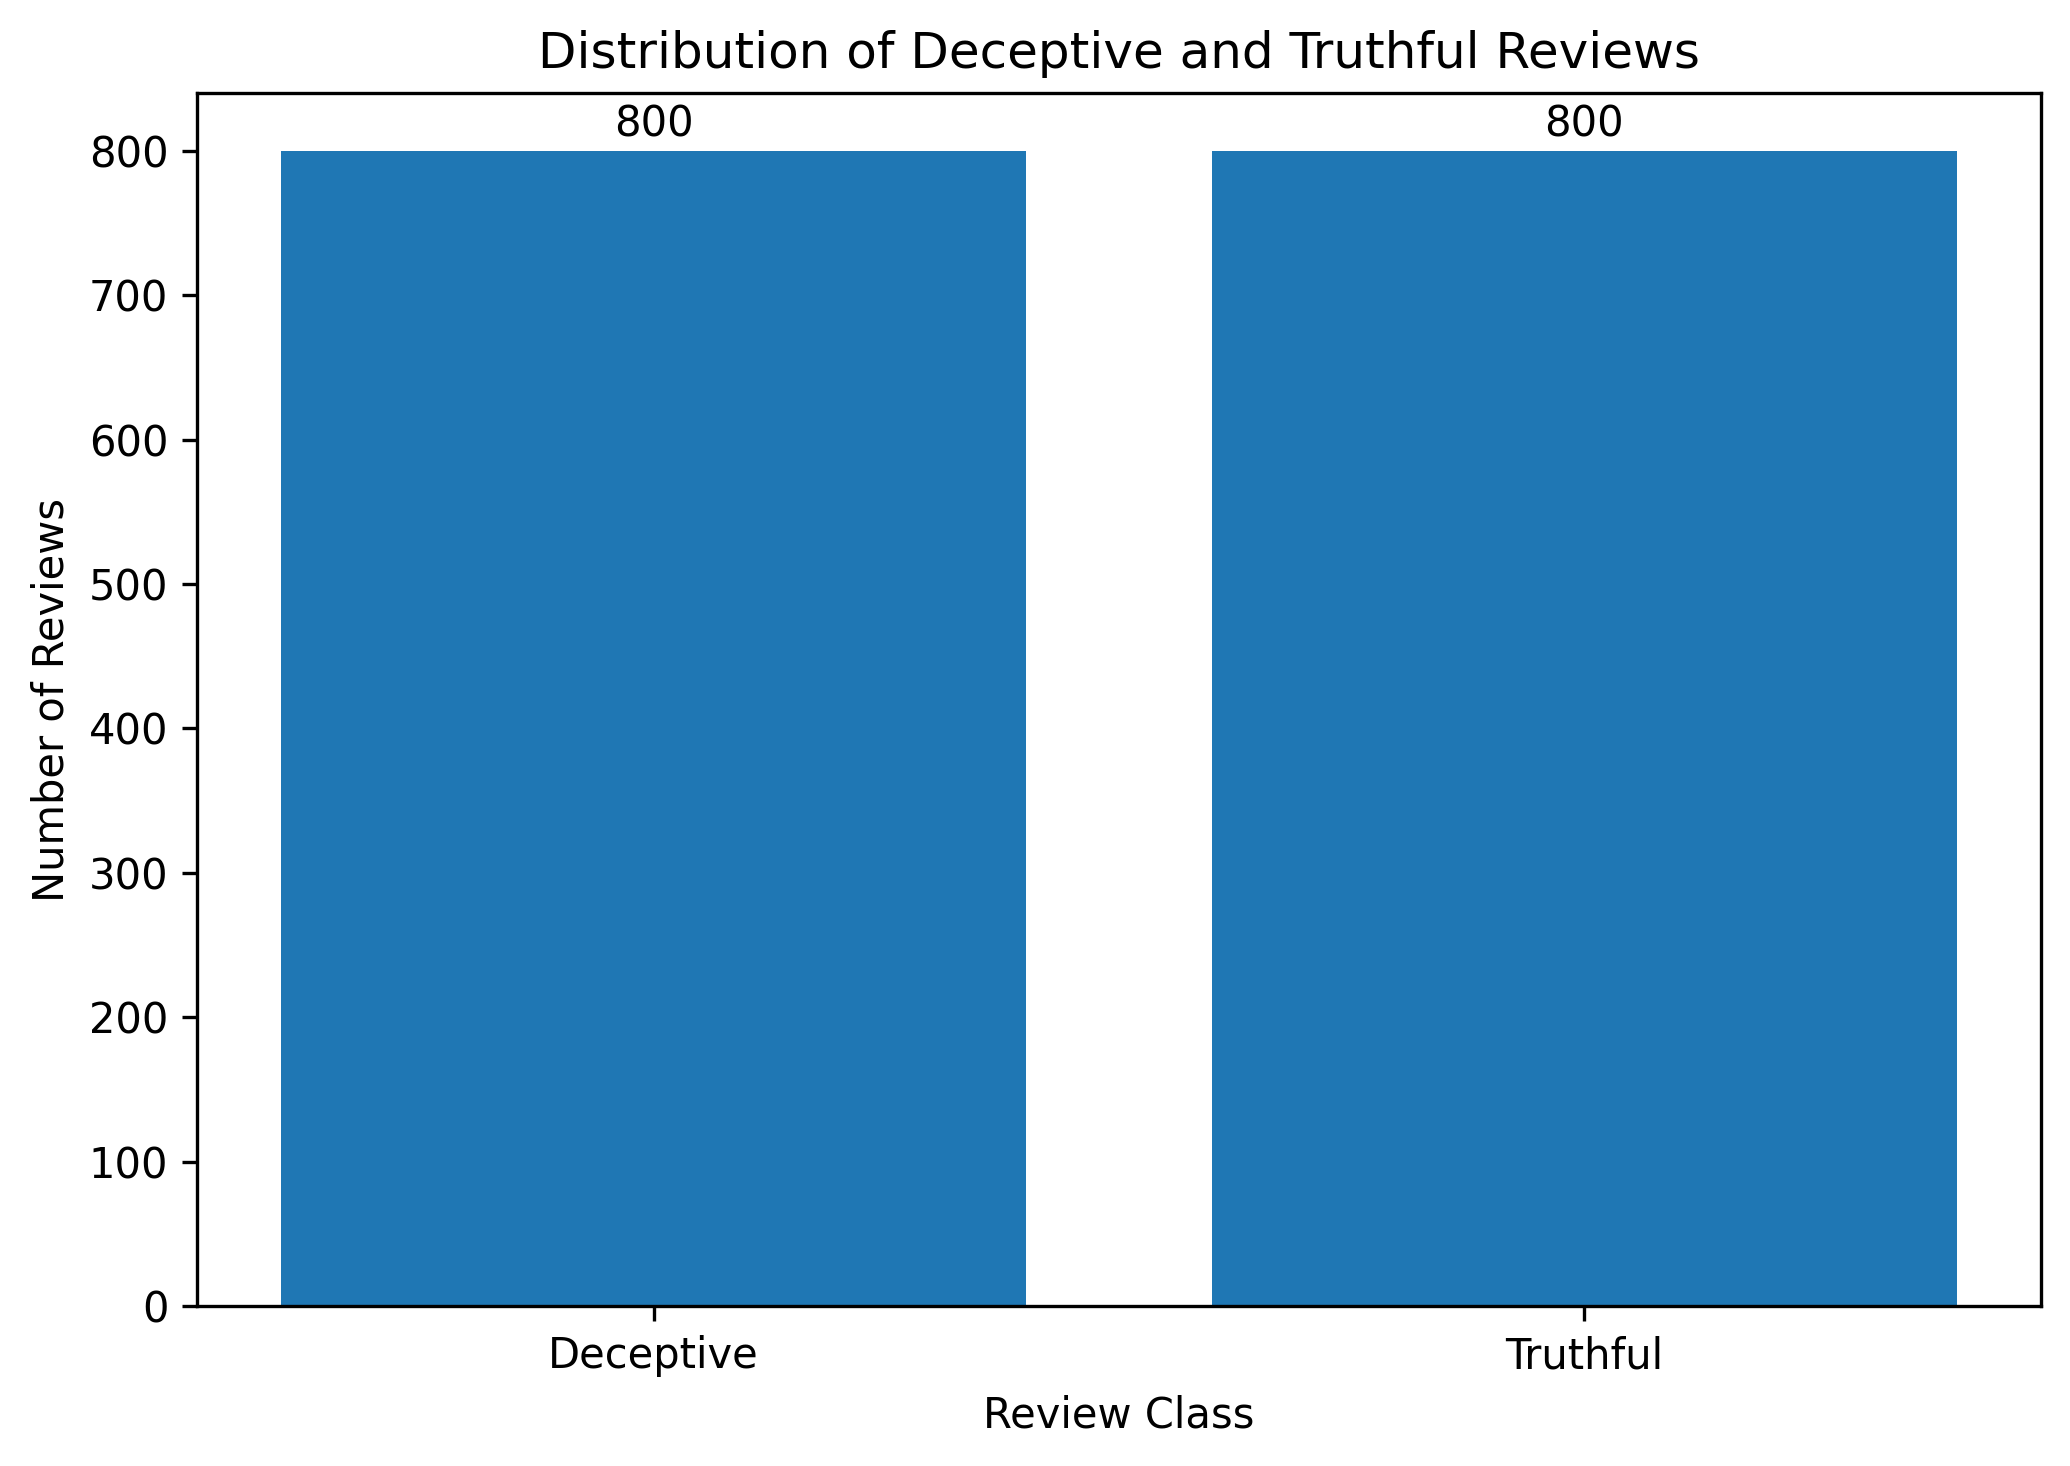
\includegraphics[width=0.75\textwidth]
    {figures/class_distribution.png}
    \caption{Distribution of Deceptive and Truthful Reviews}
    \label{fig:class_distribution}
\end{figure}

Figure~\ref{fig:class_distribution} illustrates the distribution of deceptive and truthful reviews in the dataset. The dataset contains 800 reviews in each class, confirming a balanced distribution suitable for unbiased model training.

\begin{figure}[H]
    \centering
    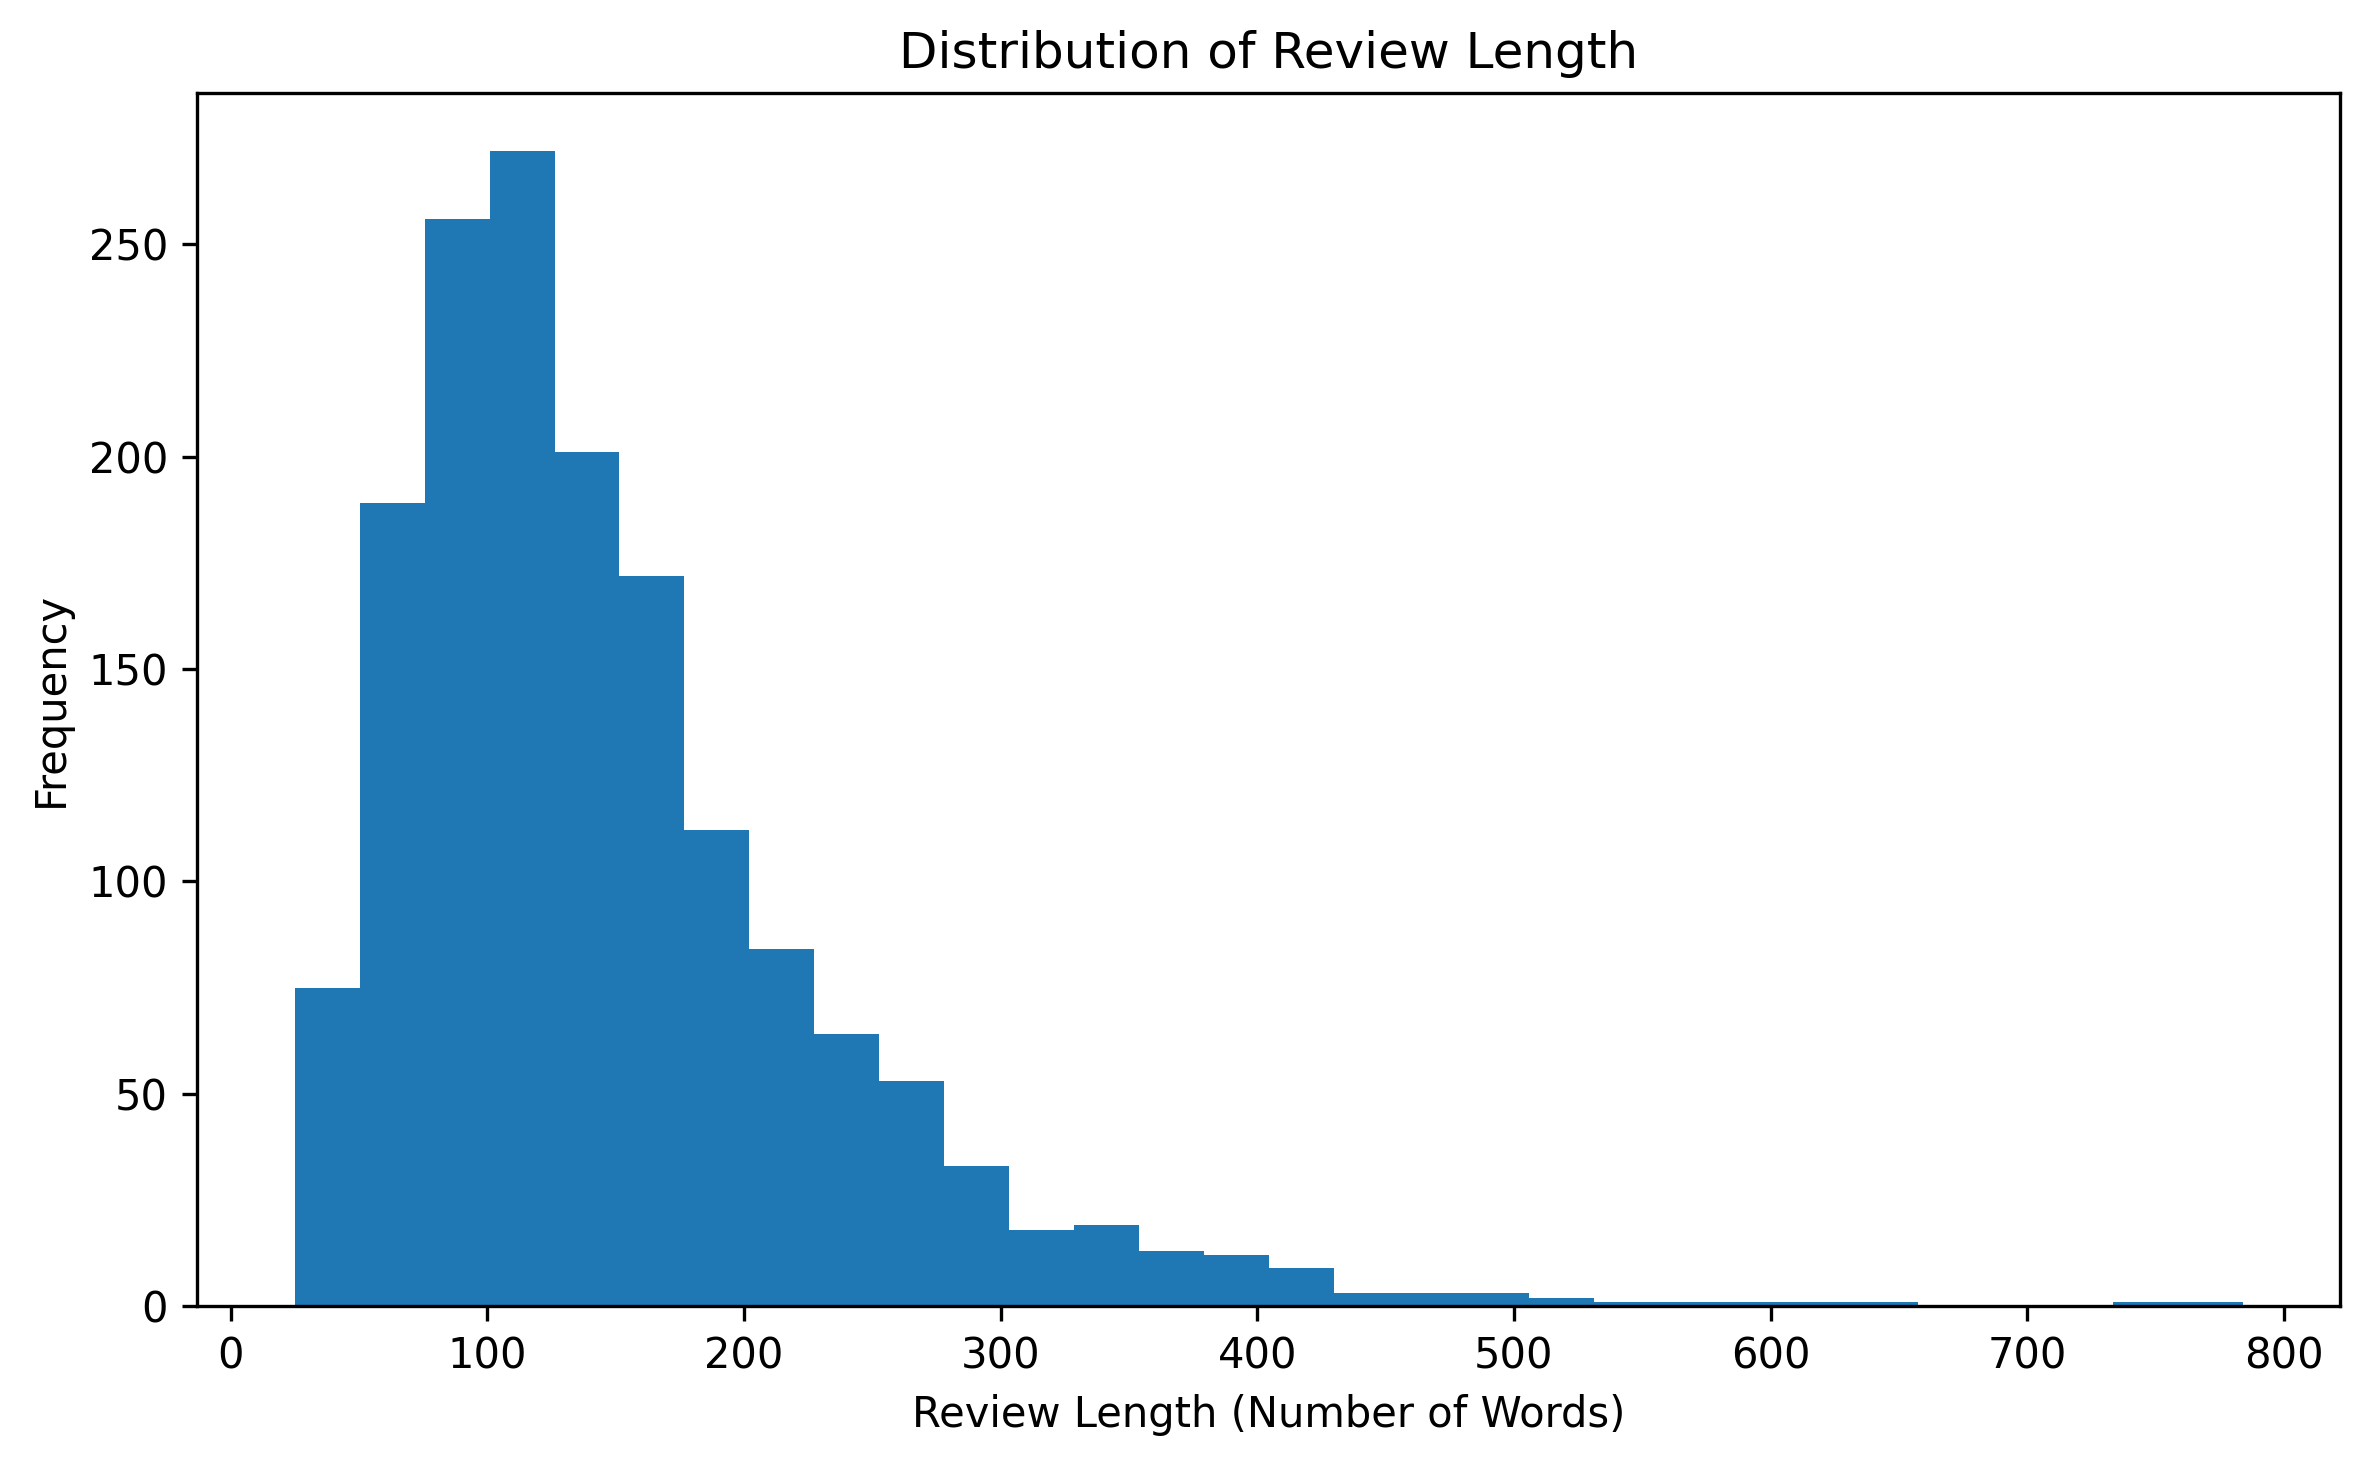
\includegraphics[width=0.85\textwidth]
    {figures/review_length_distribution.png}
    \caption{Distribution of Review Length}
    \label{fig:review_length_distribution}
\end{figure}

Figure~\ref{fig:review_length_distribution} displays the variation in review lengths across the corpus. The distribution shows the diversity in word counts between reviews, supporting the inclusion of review length and sentence count as structural linguistic features.

\subsection*{Engineered Feature Visualizations}

Following data cleaning and feature engineering, visual analyses were conducted on the VADER sentiment scores and engineered linguistic attributes to assess their discriminatory characteristics between fake and genuine reviews.

\begin{figure}[H]
    \centering
    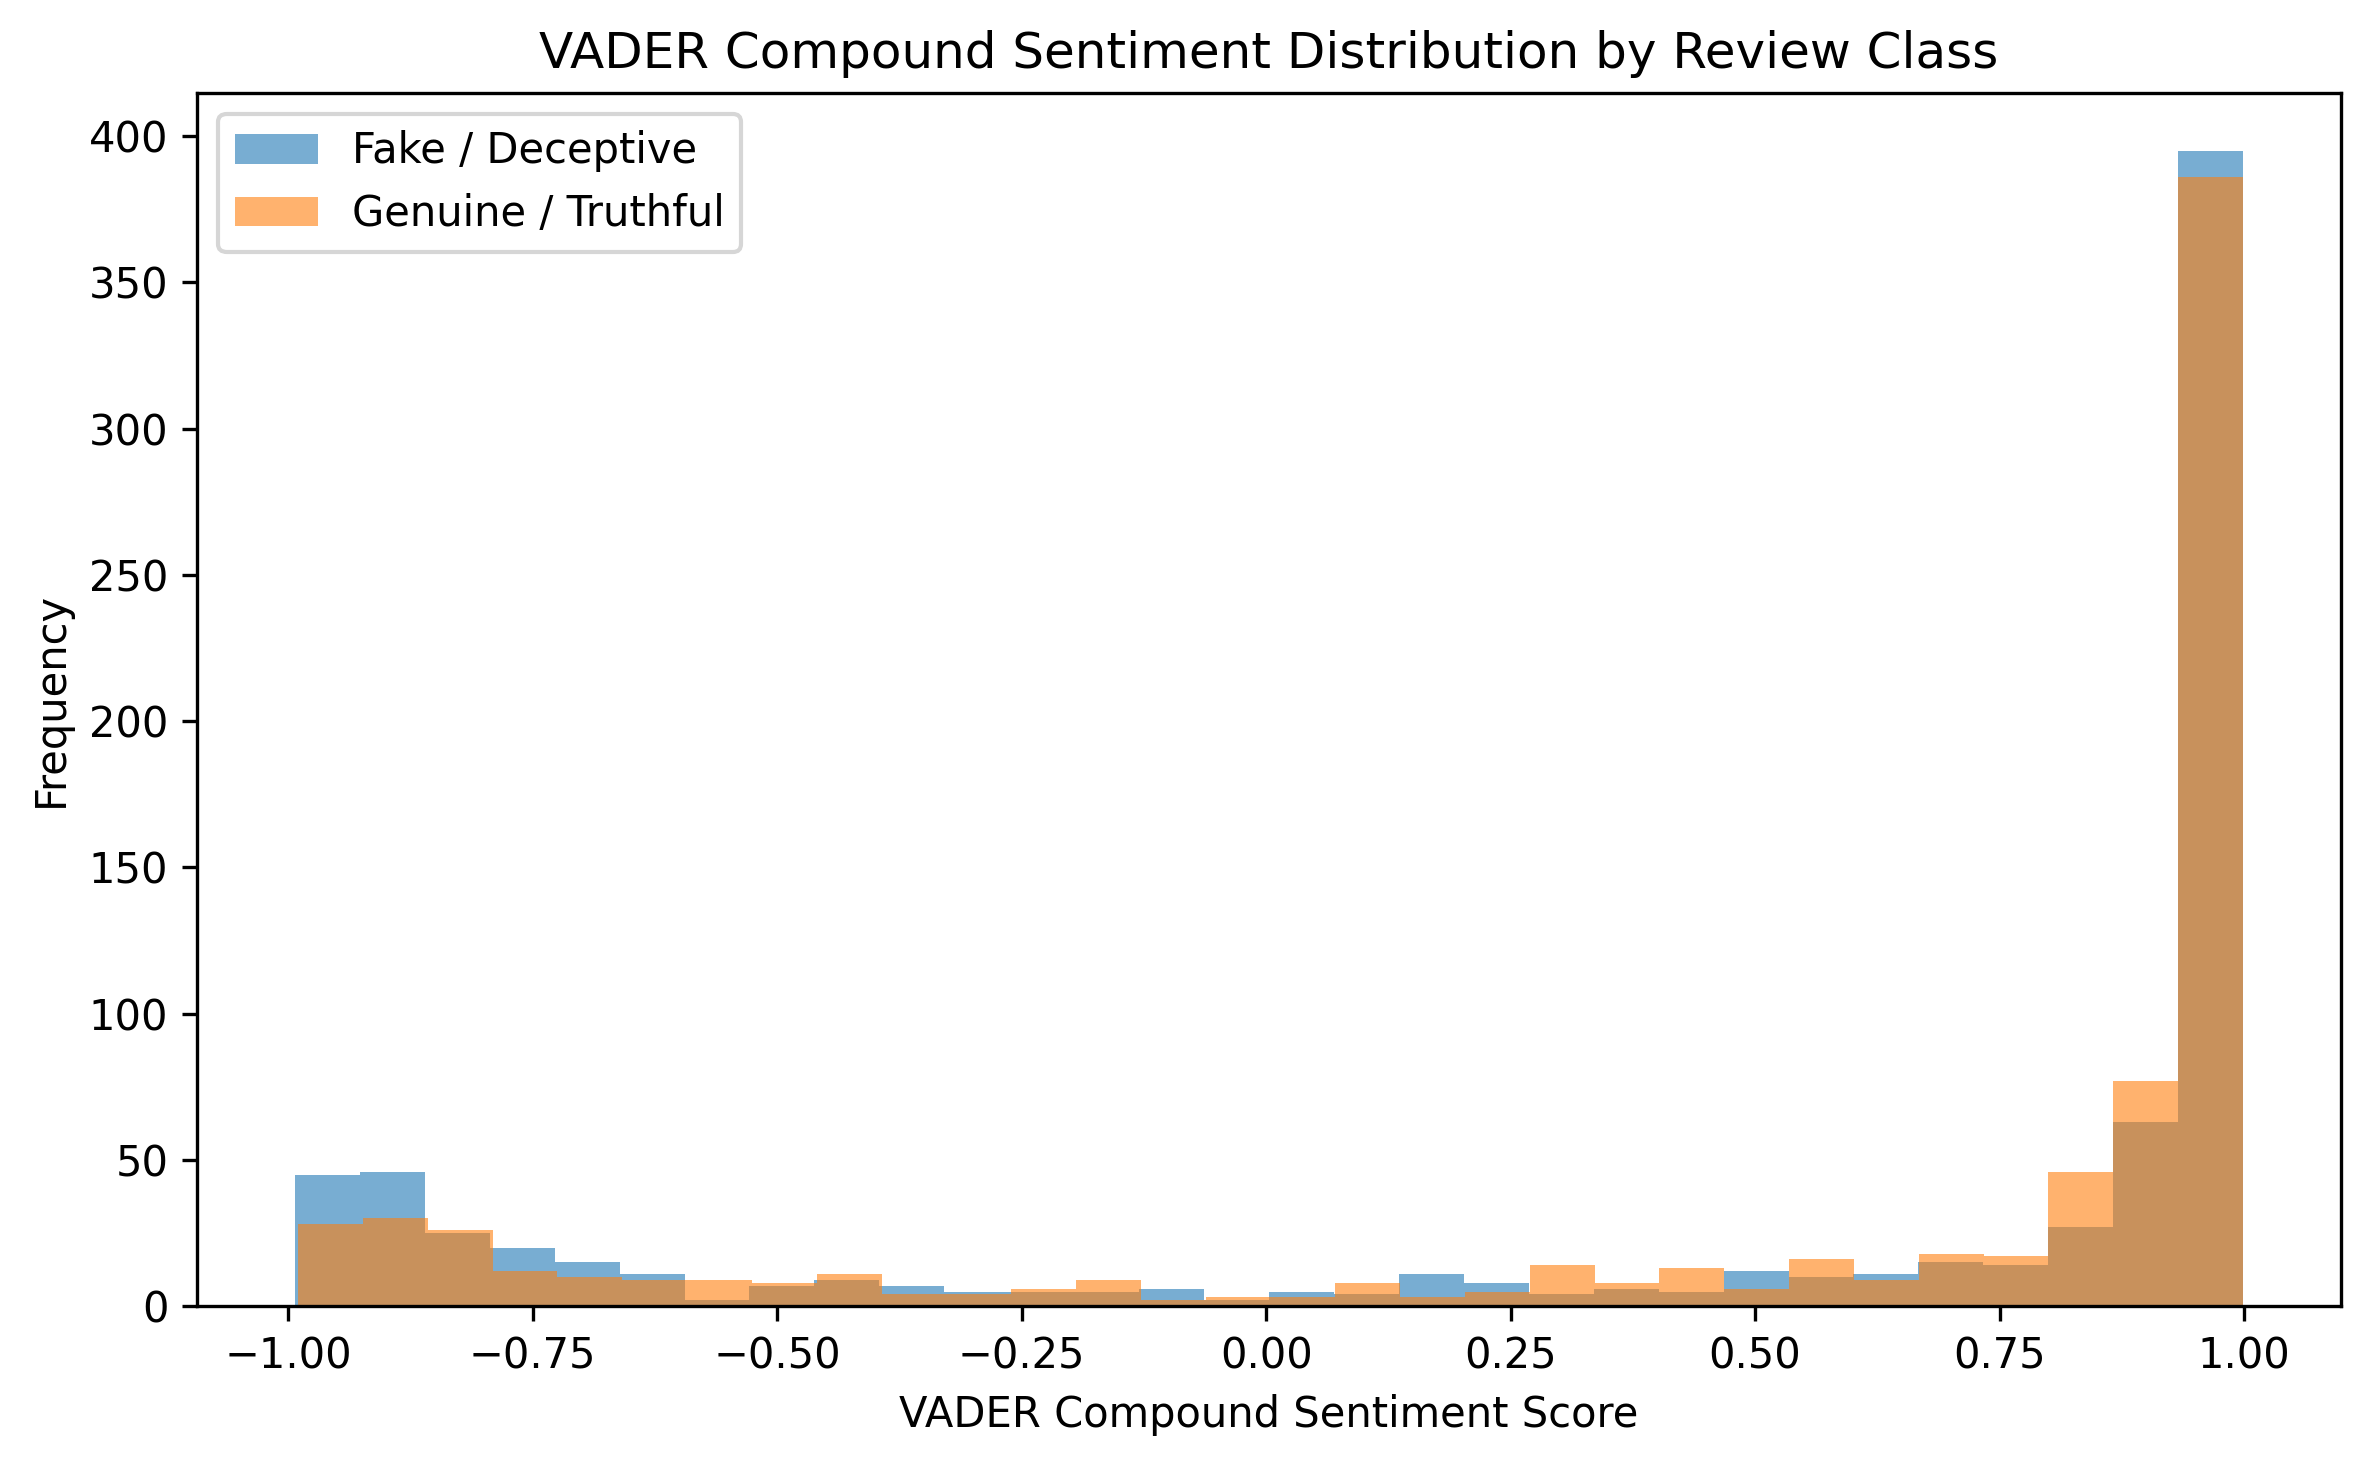
\includegraphics[width=0.83\textwidth]{figures/sentiment_distribution_by_class.png}
    \caption{VADER Compound Sentiment Distribution by Review Class}
    \label{fig:sentiment_distribution}
\end{figure}

Figure~\ref{fig:sentiment_distribution} compares the VADER compound sentiment score distributions between fake and genuine reviews. Deceptive reviews frequently exhibit exaggerated positive sentiment polarity, while genuine reviews reflect more balanced, nuanced evaluation tones.

\begin{figure}[H]
    \centering
    \includegraphics[width=0.95\textwidth]{{"figures/feature_correlation_heatmap (2)"}.png}
    \caption{Correlation Heatmap of Engineered Features}
    \label{fig:feature_correlation}
\end{figure}

Figure~\ref{fig:feature_correlation} presents the correlation heatmap of the engineered linguistic and sentiment features along with the target class label. The heatmap confirms low inter-feature collinearity while highlighting informative associations with deceptive review patterns.

% ============================================================
% 3.4 ANALYSIS OF ALGORITHMS
% ============================================================

\section{Analysis of Algorithms}

The proposed Fake Review Detection System uses supervised machine learning algorithms to classify reviews into fake and genuine classes. The input to the classifiers is constructed using four feature configurations: TF-IDF alone, TF-IDF with linguistic features, TF-IDF with VADER sentiment features, and TF-IDF with both linguistic and VADER features. Three classical machine learning algorithms are considered for classification: Logistic Regression, Linear Support Vector Machine (SVM), and Random Forest.

These algorithms are selected because they provide different approaches to binary classification. Logistic Regression provides a probabilistic classification approach, Linear SVM determines a suitable decision boundary by maximizing the separation between classes, and Random Forest uses an ensemble of decision trees to perform classification. The algorithms and feature configurations will be compared using Accuracy, Precision, Recall, F1-score, ROC--AUC, and Confusion Matrix.

\subsection{Detailed Study Report of the Proposed Algorithms}

\subsubsection*{Logistic Regression}

Logistic Regression is a supervised machine learning algorithm commonly used for binary classification problems. In the proposed system, it will be used to classify a review as either fake or genuine based on the extracted feature representation.

Logistic Regression calculates a weighted combination of the input features and converts the resulting value into a probability using the sigmoid function. The probability is then used to determine the class of the input review.

\subsubsection*{Working Principle}

Let the input feature vector be represented as

\[
\mathbf{x} = [x_1,x_2,\ldots,x_n]
\]

where each \(x_i\) represents one feature of the review. The weighted sum of the features is calculated as

\[
z = w_1x_1 + w_2x_2 + \cdots + w_nx_n + b
\]

where \(w_i\) represents the weight associated with a feature and \(b\) represents the bias.

The calculated value is passed through the sigmoid function:

\[
P(y=1|\mathbf{x}) =
\frac{1}{1+e^{-z}}
\]

The sigmoid function produces a value between 0 and 1, which can be interpreted as the probability that the review belongs to class 1.

In the proposed system, Label 1 represents a fake or deceptive review and Label 0 represents a genuine or truthful review. Therefore, the classification rule is:

\[
P(y=1|\mathbf{x}) \geq 0.5
\Rightarrow \text{Fake / Deceptive Review}
\]

\[
P(y=1|\mathbf{x}) < 0.5
\Rightarrow \text{Genuine / Truthful Review}
\]

The model parameters are learned by minimizing the binary cross-entropy loss:

\[
L =
-\left[y\log(p)+(1-y)\log(1-p)\right]
\]

where \(y\) is the actual class and \(p\) is the predicted probability.

During training, the model parameters are optimized to reduce the classification loss. The displayed expression represents the loss for one sample; training minimizes the loss over the training data, with regularization where applicable.

\subsubsection*{Application in the Proposed System}

In the proposed system, Logistic Regression will be examined using different feature configurations based on TF-IDF, linguistic characteristics, and VADER sentiment scores.

The TF-IDF representation consists of unigram and bigram features with a maximum of 10,000 features. Six linguistic features are extracted from the reviews: Review Length, Sentence Count, Average Word Length, Exclamation Count, Question Count, and Capital Count.

In addition, four sentiment-based features are extracted using VADER: Positive, Negative, Neutral, and Compound sentiment scores.

Each feature configuration will be supplied separately to the Logistic Regression classifier for training and comparison. The model will use a regularization parameter of \(C=1.0\) and a maximum of 2000 iterations, as specified in the model-building section. The implementation uses regularized binary classification.

\subsubsection*{Advantages}

\begin{itemize}
    \item Simple and efficient for binary classification.
    \item Provides probability-based predictions.
    \item Works effectively with high-dimensional TF-IDF features.
    \item Easy to interpret compared with more complex models.
    \item Requires relatively low computational resources.
\end{itemize}

\subsubsection*{Limitations}

\begin{itemize}
    \item Assumes a linear decision boundary between the classes.
    \item May not capture complex non-linear relationships between features.
    \item Performance can depend on the quality of the feature representation.
\end{itemize}

\subsubsection*{Activity Diagram}

The activity diagram for Logistic Regression summarizes the conceptual stages of model training and prediction. The optimization steps represent the learning process rather than a specific solver implementation.

Figure~\ref{fig:logistic_activity} illustrates the training and prediction process of Logistic Regression. During training, the model will initialize its parameters, calculate the linear score, apply the sigmoid function, calculate the loss, and update the parameters until convergence. After training, the model will calculate the probability for a new review and classify it as fake or genuine using a threshold of 0.5. In accordance with the dataset labels, Label 1 represents a fake or deceptive review, while Label 0 represents a genuine or truthful review.

\begin{figure}[H]
\centering

\begin{tikzpicture}[
    node distance=4mm,
    >=Stealth,
    every node/.style={font=\scriptsize},
    startstop/.style={
        ellipse,
        draw,
        minimum width=18mm,
        minimum height=5mm,
        align=center
    },
    process/.style={
        rectangle,
        draw,
        rounded corners=1pt,
        minimum width=36mm,
        minimum height=6mm,
        align=center
    },
    decision/.style={
        diamond,
        draw,
        aspect=2.2,
        inner sep=1pt,
        align=center
    },
    arrow/.style={
        ->,
        thick
    }
]

\node (start) [startstop] {START};

\node (input) [process, below=of start]
{Input Training Feature Matrix};

\node (init) [process, below=of input]
{Initialize Weights and Bias};

\node (linear) [process, below=of init]
{Calculate Linear Score\\
\(z=\mathbf{w}^{T}\mathbf{x}+b\)};

\node (sigmoid) [process, below=of linear]
{Apply Sigmoid Function};

\node (loss) [process, below=of sigmoid]
{Calculate Prediction and Loss};

\node (update) [process, below=of loss]
{Update Weights and Bias};

\node (converged) [decision, below=of update]
{Converged?};

\node (trained) [process, below=of converged, yshift=-3mm]
{Trained Logistic Regression Model};

\node (newinput) [process, below=of trained]
{Input New Review Feature Vector};

\node (prob) [process, below=of newinput]
{Calculate Prediction Probability};

\node (threshold) [decision, below=of prob]
{Probability \(\geq 0.5\)?};

\node (fake) [process, below left=5mm and 10mm of threshold]
{Fake / Deceptive\\(Label = 1)};

\node (genuine) [process, below right=5mm and 10mm of threshold]
{Genuine / Truthful\\(Label = 0)};

\node (end) [startstop, below=18mm of threshold]
{END};

\draw [arrow] (start) -- (input);
\draw [arrow] (input) -- (init);
\draw [arrow] (init) -- (linear);
\draw [arrow] (linear) -- (sigmoid);
\draw [arrow] (sigmoid) -- (loss);
\draw [arrow] (loss) -- (update);
\draw [arrow] (update) -- (converged);

\draw [arrow] (converged) -- node[right] {Yes} (trained);

\draw [arrow] (converged.west) -- ++(-12mm,0)
    |- node[pos=0.25,left] {No} (linear.west);

\draw [arrow] (trained) -- (newinput);
\draw [arrow] (newinput) -- (prob);
\draw [arrow] (prob) -- (threshold);

\draw [arrow] (threshold) -- node[above left] {Yes} (fake);
\draw [arrow] (threshold) -- node[above right] {No} (genuine);

\draw [arrow] (fake) |- (end);
\draw [arrow] (genuine) |- (end);

\end{tikzpicture}

\caption{Activity Diagram of Logistic Regression}
\label{fig:logistic_activity}
\end{figure}


% ============================================================
% RANDOM FOREST
% ============================================================

\subsubsection*{Random Forest}

Random Forest is an ensemble machine learning algorithm that combines multiple decision trees to perform classification. Instead of depending on a single decision tree, Random Forest creates several decision trees and combines their predictions to obtain the final classification.

The use of multiple trees reduces the dependence on an individual decision tree and allows the model to capture different patterns present in the training data. In the proposed system, Random Forest will be used to classify reviews as either fake/deceptive or genuine/truthful.

\subsubsection*{Working Principle}

Random Forest creates multiple decision trees using different bootstrap samples of the training data. For each tree, a randomly selected subset of features is considered while constructing the tree.

If the forest contains \(T\) decision trees, each tree produces a prediction:

\[
h_1(\mathbf{x}),h_2(\mathbf{x}),\ldots,h_T(\mathbf{x})
\]

The final prediction is obtained using majority voting:

\[
\hat{y}
=
\operatorname{mode}
\left\{
h_1(\mathbf{x}),
h_2(\mathbf{x}),
\ldots,
h_T(\mathbf{x})
\right\}
\]

The class receiving the highest number of votes from the individual trees becomes the final predicted class.

In the proposed system, Label 1 represents a fake or deceptive review, while Label 0 represents a genuine or truthful review.

\subsubsection*{Training Process}

The training process begins by generating bootstrap samples from the training data. A decision tree is then constructed from each sample. During tree construction, random subsets of features are considered at different nodes. This process is repeated until the required number of trees is created.

In the model-building configuration, the Random Forest classifier will use 300 decision trees. The predictions from these trees will be combined using majority voting to obtain the final classification.

\subsubsection*{Application in the Proposed System}

The Random Forest classifier will be evaluated using the same four feature configurations as the other proposed algorithms, allowing comparison across TF-IDF, linguistic, and sentiment-based representations.

The TF-IDF representation consists of unigram and bigram features with a maximum of 10,000 features. Six linguistic features are extracted from the reviews: Review Length, Sentence Count, Average Word Length, Exclamation Count, Question Count, and Capital Count.

In addition, four sentiment-based features are extracted using VADER: Positive, Negative, Neutral, and Compound sentiment scores.

Each feature configuration will be provided separately to the Random Forest classifier. The trained trees will combine their predictions to classify a new review as fake/deceptive or genuine/truthful.

\subsubsection*{Advantages}

\begin{itemize}
    \item Combines multiple decision trees to improve classification stability.
    \item Can capture non-linear relationships between features.
    \item Is less sensitive to individual decision tree errors.
    \item Can handle a large number of input features.
    \item Provides an ensemble-based classification approach.
\end{itemize}

\subsubsection*{Limitations}

\begin{itemize}
    \item Requires more computational resources than simpler linear models.
    \item A large number of trees can increase training and prediction time.
    \item The complete ensemble is more difficult to interpret than a single decision tree.
\end{itemize}

\subsubsection*{Activity Diagram}

The activity diagram for Random Forest represents the process of generating multiple decision trees and combining their predictions to obtain the final class.

Figure~\ref{fig:random_forest_activity} shows the main training and prediction stages of Random Forest. Bootstrap samples and random feature subsets are used to construct multiple decision trees. After the required number of trees is completed, a new review is passed through the individual trees and their predictions are combined using majority voting to obtain the final classification. In the proposed system, the final classification will represent either a fake/deceptive review (Label 1) or a genuine/truthful review (Label 0).
\begin{figure}[H]
\centering

\begin{tikzpicture}[
    node distance=4mm,
    >=Stealth,
    every node/.style={font=\scriptsize},
    startstop/.style={
        ellipse,
        draw,
        minimum width=18mm,
        minimum height=5mm,
        align=center
    },
    process/.style={
        rectangle,
        draw,
        rounded corners=1pt,
        minimum width=36mm,
        minimum height=6mm,
        align=center
    },
    decision/.style={
        diamond,
        draw,
        aspect=2.2,
        inner sep=1pt,
        align=center
    },
    arrow/.style={
        ->,
        thick
    }
]

\node (start) [startstop] {START};

\node (input) [process, below=of start]
{Input Training Feature Matrix};

\node (bootstrap) [process, below=of input]
{Generate Bootstrap Sample};

\node (features) [process, below=of bootstrap]
{Select Random Feature Subset};

\node (tree) [process, below=of features]
{Build Decision Tree};

\node (more) [decision, below=of tree]
{More Trees?};

\node (forest) [process, below=of more, yshift=-3mm]
{Forest of Decision Trees Completed};

\node (newinput) [process, below=of forest]
{Input New Review Feature Vector};

\node (predict) [process, below=of newinput]
{Obtain Prediction from Each Tree};

\node (vote) [process, below=of predict]
{Apply Majority Voting};

\node (classify) [decision, below=of vote]
{Final Class?};

\node (fake) [process, below left=5mm and 10mm of classify]
{Fake / Deceptive\\(Label = 1)};

\node (genuine) [process, below right=5mm and 10mm of classify]
{Genuine / Truthful\\(Label = 0)};

\node (end) [startstop, below=18mm of classify]
{END};

\draw [arrow] (start) -- (input);
\draw [arrow] (input) -- (bootstrap);
\draw [arrow] (bootstrap) -- (features);
\draw [arrow] (features) -- (tree);
\draw [arrow] (tree) -- (more);

\draw [arrow] (more) -- node[right] {No} (forest);

\draw [arrow] (more.west) -- ++(-12mm,0)
    |- node[pos=0.25,left] {Yes} (bootstrap.west);

\draw [arrow] (forest) -- (newinput);
\draw [arrow] (newinput) -- (predict);
\draw [arrow] (predict) -- (vote);
\draw [arrow] (vote) -- (classify);

\draw [arrow] (classify) -- node[above left] {Fake} (fake);
\draw [arrow] (classify) -- node[above right] {Genuine} (genuine);

\draw [arrow] (fake) |- (end);
\draw [arrow] (genuine) |- (end);

\end{tikzpicture}

\caption{Activity Diagram of Random Forest}
\label{fig:random_forest_activity}
\end{figure}



% ============================================================
% SUPPORT VECTOR MACHINE
% ============================================================
\subsubsection*{Linear Support Vector Machine (Linear SVM)}

Linear Support Vector Machine (Linear SVM) is a supervised machine learning algorithm used for binary classification. It identifies a linear decision boundary that separates two classes while maximizing the distance between the boundary and the closest training samples.

The proposed system uses Linear SVM because TF-IDF produces a high-dimensional and sparse feature representation, which can also be combined with linguistic or sentiment-based features. Linear SVM is suitable for text classification because it can efficiently operate on high-dimensional and sparse feature representations.

\subsubsection*{Working Principle}

For a linear SVM, the decision boundary is represented by:

\[
\mathbf{w}^{T}\mathbf{x}+b=0
\]

where \(\mathbf{w}\) represents the weight vector, \(\mathbf{x}\) represents the input feature vector, and \(b\) represents the bias.

The decision function is given by:

\[
f(\mathbf{x})=\mathbf{w}^{T}\mathbf{x}+b
\]

The predicted class is determined from the sign of the decision function. In the proposed system, Label 1 represents a fake or deceptive review, while Label 0 represents a genuine or truthful review. Therefore, the classification rule is:

\[
f(\mathbf{x}) \geq 0
\Rightarrow \text{Fake / Deceptive Review}
\]

\[
f(\mathbf{x}) < 0
\Rightarrow \text{Genuine / Truthful Review}
\]

The objective of Linear SVM is to identify a separating hyperplane with a large margin while allowing classification errors when necessary. The margin for a linear SVM is related to the magnitude of the weight vector:

\[
\text{Margin}=\frac{2}{\|\mathbf{w}\|}
\]

For a hard-margin formulation, the optimization problem can be written as:

\[
\min_{\mathbf{w},b}
\frac{1}{2}\|\mathbf{w}\|^2
\]

subject to:

\[
y_i(\mathbf{w}^{T}\mathbf{x}_i+b)\geq1
\]

where \(y_i\) is the signed class label in \(\{-1,+1\}\). This is the mathematical convention used for the margin constraint; the original dataset labels remain 0 (genuine) and 1 (fake) and are handled by the classifier internally.

For practical datasets, Linear SVM uses a soft-margin formulation with regularization parameter \(C\), which balances a large margin against classification errors. The hard-margin equations above are provided to explain the underlying principle.

\subsubsection*{Support Vectors}

Support vectors are the training samples that are closest to the decision boundary. These samples play an important role in determining the position of the separating hyperplane. Changes in the support vectors can affect the position of the decision boundary, whereas samples that are far from the boundary have less direct influence on it.

\subsubsection*{Application in the Proposed System}

In the proposed system, \texttt{LinearSVC} will be evaluated using four feature configurations constructed from TF-IDF, linguistic features, and VADER sentiment scores.

The TF-IDF representation consists of unigram and bigram features with a maximum of 10,000 features. Six linguistic features are extracted from the reviews: Review Length, Sentence Count, Average Word Length, Exclamation Count, Question Count, and Capital Count.

In addition, four sentiment-based features are extracted using VADER: Positive, Negative, Neutral, and Compound sentiment scores.

Each feature configuration will be supplied separately to \texttt{LinearSVC}. The regularization parameter will be set to \(C=1.0\); the maximum number of iterations will be set to 2000. The trained model will calculate a decision value for an unseen review and use its sign to classify the review as fake/deceptive or genuine/truthful.

\subsubsection*{Advantages}

\begin{itemize}
    \item Effective for high-dimensional feature spaces.
    \item Works well with sparse TF-IDF representations.
    \item Uses a clear linear decision boundary for classification.
    \item Linear SVM is computationally suitable for text feature spaces.
\end{itemize}

\subsubsection*{Limitations}

\begin{itemize}
    \item Does not directly provide probability estimates in the same way as Logistic Regression.
    \item Performance depends on the selected model parameters and feature representation.
    \item A linear SVM may not capture complex non-linear relationships between features.
\end{itemize}

\subsubsection*{Activity Diagram}

The activity diagram for Linear SVM represents the process of learning the separating hyperplane and using it to classify a new review.

\begin{figure}[H]
\centering

\begin{tikzpicture}[
    node distance=4mm,
    >=Stealth,
    every node/.style={font=\scriptsize},
    startstop/.style={
        ellipse,
        draw,
        minimum width=18mm,
        minimum height=5mm,
        align=center
    },
    process/.style={
        rectangle,
        draw,
        rounded corners=1pt,
        minimum width=36mm,
        minimum height=6mm,
        align=center
    },
    decision/.style={
        diamond,
        draw,
        aspect=2.2,
        inner sep=1pt,
        align=center
    },
    arrow/.style={
        ->,
        thick
    }
]

\node (start) [startstop] {START};

\node (input) [process, below=of start]
{Input Training Feature Matrix};

\node (boundary) [process, below=of input]
{Determine Linear Decision Hyperplane};

\node (margin) [process, below=of boundary]
{Calculate Margin};

\node (support) [process, below=of margin]
{Identify Support Vectors};

\node (optimize) [process, below=of support]
{Optimize Hyperplane and Margin};

\node (converged) [decision, below=of optimize]
{Converged?};

\node (trained) [process, below=of converged, yshift=-3mm]
{Trained Linear SVM Model};

\node (newinput) [process, below=of trained]
{Input New Review Feature Vector};

\node (decisionvalue) [process, below=of newinput]
{Calculate Decision Value\\
\(f(\mathbf{x})=\mathbf{w}^{T}\mathbf{x}+b\)};

\node (classify) [decision, below=of decisionvalue]
{\(f(\mathbf{x})\geq0\)?};

\node (fake) [process, below left=5mm and 10mm of classify]
{Fake / Deceptive\\(Label = 1)};

\node (genuine) [process, below right=5mm and 10mm of classify]
{Genuine / Truthful\\(Label = 0)};

\node (end) [startstop, below=18mm of classify]
{END};

\draw [arrow] (start) -- (input);
\draw [arrow] (input) -- (boundary);
\draw [arrow] (boundary) -- (margin);
\draw [arrow] (margin) -- (support);
\draw [arrow] (support) -- (optimize);
\draw [arrow] (optimize) -- (converged);

\draw [arrow] (converged) -- node[right] {Yes} (trained);

\draw [arrow] (converged.west) -- ++(-12mm,0)
    |- node[pos=0.25,left] {No} (optimize.west);

\draw [arrow] (trained) -- (newinput);
\draw [arrow] (newinput) -- (decisionvalue);
\draw [arrow] (decisionvalue) -- (classify);

\draw [arrow] (classify) -- node[above left] {Yes} (fake);
\draw [arrow] (classify) -- node[above right] {No} (genuine);

\draw [arrow] (fake) |- (end);
\draw [arrow] (genuine) |- (end);

\end{tikzpicture}

\caption{Activity Diagram of Linear Support Vector Machine}
\label{fig:svm_activity}
\end{figure}

Figure~\ref{fig:svm_activity} represents the main stages of the Linear SVM algorithm. The model learns a linear separating hyperplane by optimizing a regularized classification objective. The diagram presents the margin and support vectors conceptually. After training, the decision function is calculated for a new review and the sign of the decision value determines the predicted class. In accordance with the dataset labels, a non-negative decision value corresponds to a fake/deceptive review (Label 1), while a negative decision value corresponds to a genuine/truthful review (Label 0).

\section{Project Pipeline}

\subsection{Project Pipeline Diagram and Development Plan}

The proposed Fake Review Detection System follows a structured machine learning pipeline that transforms raw hotel review data into a suitable feature representation for classifying reviews as fake/deceptive or genuine/truthful. The major stages include dataset loading, EDA, preprocessing, feature extraction, feature selection, model training, evaluation, and prediction.

Initially, the Ott Deceptive Opinion Spam Corpus is loaded into the system. It contains hotel review text, ratings, and class labels. The review text is used for feature extraction, while the label is used as the target variable. Label 1 represents fake/deceptive reviews, whereas Label 0 represents genuine/truthful reviews.

Exploratory Data Analysis (EDA) is performed to understand the dataset characteristics, including class distribution and review length. The dataset is also checked for missing values and duplicate records.

The review text is preprocessed using NLP techniques, including HTML tag removal, lowercase conversion, removal of URLs, numbers, punctuation, and special characters, followed by tokenization, English stop-word removal, and lemmatization.

Feature engineering is then performed using TF-IDF with unigram and bigram features, with a maximum of 10,000 features. Six linguistic features are extracted: Review Length, Sentence Count, Average Word Length, Exclamation Count, Question Count, and Capital Count. VADER sentiment analysis provides four additional features: Positive, Negative, Neutral, and Compound scores.

Feature selection is performed to retain relevant features for classification. The dataset is divided using a stratified 80:20 train-test split. The TF-IDF vectorizer is fitted only on the training data and then applied to both training and testing data. The selected linguistic and sentiment features are combined with the TF-IDF representation to form the final feature matrix.

The combined training features are used to train three classifiers: Logistic Regression, Linear SVM, and Random Forest. Logistic Regression is configured with $C=1.0$ and a maximum of 2000 iterations, Linear SVM uses a maximum of 2000 iterations, and Random Forest uses 300 decision trees.

The trained models are evaluated using Accuracy, Precision, Recall, F1-score, ROC--AUC, and Confusion Matrix. Their performance is compared, and the best-performing model is selected based on the overall evaluation results.

Finally, the selected model is deployed to classify unseen reviews. A new review undergoes the same preprocessing and feature extraction steps before being supplied to the trained model, which predicts whether it is fake/deceptive (Label 1) or genuine/truthful (Label 0).

\begin{figure}[H]
    \centering
    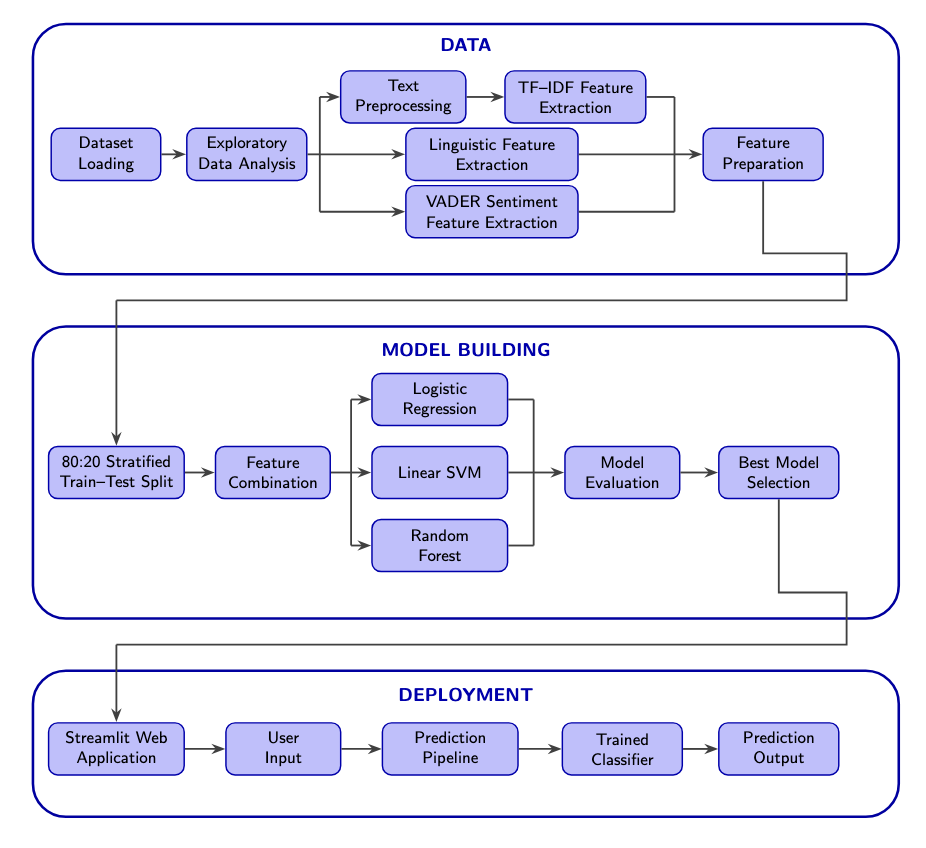
\includegraphics[width=0.95\textwidth]{figures/project_pipeline.png}
    \caption{Project Pipeline}
    \label{fig:project_pipeline}
\end{figure}

\noindent\textbf{Project Development Plan and Timeline}

The project timeline outlines the major activities planned for the development of the Fake Review Detection System, from dataset analysis and text preprocessing to feature extraction, machine learning model development, evaluation, application implementation, testing, and final submission. The activities are organized according to the common project schedule and presentation milestones.

The planned project activities are:

\begin{table}[H]
\centering
\renewcommand{\arraystretch}{1.5}
\setlength{\tabcolsep}{8pt}

\begin{tabularx}{\textwidth}{|>{\raggedright\arraybackslash}p{3.5cm}|X|}
\hline
\textbf{Period / Date} & \textbf{Planned Activity} \\
\hline

Week 1--2 &
Dataset Collection, Exploratory Data Analysis and Initial Text Preprocessing \\
\hline

21.07.2026 &
Project Proposal Approval \\
\hline

Week 3 &
Feature Extraction and Feature Dataset Preparation using TF-IDF, Linguistic and VADER Sentiment Features \\
\hline

Week 4 &
Feature Analysis, Feature Selection and Visualization \\
\hline

Week 5 &
Machine Learning Pipeline Preparation and Analysis of Selected Algorithms \\
\hline

Week 6 &
Finalization of Preprocessing, Feature Engineering and Model Implementation Setup \\
\hline

09.09.2026 &
First Project Presentation -- Sprint Release I \\
\hline

Week 8 &
Model Training using Logistic Regression, Linear SVM and Random Forest \\
\hline

18.09.2026 &
Sprint Release II \\
\hline

Week 9 &
Model Performance Evaluation, Model Comparison and Selection of the Best-Performing Model \\
\hline

Week 10 &
Web Interface Development, Review Input Interface and CSV Upload/Prediction Implementation \\
\hline

29.09.2026 -- 30.09.2026 &
Interim Project Presentation \\
\hline

Week 11 &
Prediction Result Interface, Classification Report Generation, System Integration, Testing and Refinement \\
\hline

05.10.2026 &
Project Execution, Report and PPT Preparation \\
\hline

09.10.2026 &
Sprint Release III \\
\hline

22.10.2026 -- 23.10.2026 &
Final Project Presentation \\
\hline

30.10.2026 &
Final Report Submission \\
\hline

\end{tabularx}

\caption{Project Timeline}
\label{tab:project_timeline}
\end{table}

\section{Feasibility Analysis}

Feasibility analysis evaluates whether the proposed Fake Review Detection System can be successfully developed using the available resources, technologies, and project duration. The system is analysed from technical, operational, economic, and schedule perspectives.

\subsection{Technical Feasibility}

The proposed system is technically feasible as it uses established Natural Language Processing techniques and classical machine learning algorithms. The Ott Deceptive Opinion Spam Corpus provides labelled hotel reviews suitable for supervised binary classification.

Python and commonly available libraries are used for data processing, text preprocessing, feature extraction, sentiment analysis, and machine learning. TF-IDF is used for text representation, while VADER provides sentiment-based features. Linguistic features are also extracted from the reviews. Logistic Regression, Linear SVM, and Random Forest will be implemented using Scikit-learn. NLTK is used for NLP preprocessing and VADER, while Pandas, NumPy, and Matplotlib support data processing and visualization.

Therefore, the required software tools and computational resources are available, making the system technically feasible.

\subsection{Operational Feasibility}

The proposed system is operationally feasible because the review classification process can be automated after model training. A new review can pass through the same preprocessing and feature extraction pipeline before being supplied to the trained classifier.

The system provides a simple classification outcome indicating whether a review is fake/deceptive or genuine/truthful. This can assist in identifying potentially deceptive reviews with minimal manual intervention.

\subsection{Economic Feasibility}

The proposed system is economically feasible because it uses a publicly available dataset, open-source programming language, and freely available machine learning and NLP libraries.

Python, Pandas, NumPy, NLTK, Scikit-learn, and Matplotlib are freely available, eliminating the need for specialised commercial software. Therefore, the overall development cost is low and suitable for an academic project.

\subsection{Schedule Feasibility}

The proposed project is feasible within the available academic project duration. The major stages include literature review, dataset analysis, preprocessing, feature engineering, feature selection, model development, model evaluation, testing, documentation, and final report preparation.

The use of established NLP techniques and classical machine learning algorithms reduces implementation complexity and supports timely completion. Therefore, the proposed Fake Review Detection System can be completed within the planned project schedule.

\section{System Environment}

The system environment specifies the software tools,
libraries, and hardware resources required for the
development and implementation of the proposed Fake
Review Detection System. The project uses standard
computing resources for data processing, text
preprocessing, feature extraction, model development,
evaluation, and visualization.

\subsection{Software Environment}

The software environment consists of Python and
open-source libraries for data processing, Natural
Language Processing, machine learning, sentiment
analysis, and visualization. Google Colab is used
for model development and experimentation, while
Visual Studio Code supports application development.

\begin{table}[H]
\centering

\renewcommand{\arraystretch}{1.4}
\setlength{\tabcolsep}{10pt}

\begin{tabular}{|
>{\raggedright\arraybackslash}p{3.8cm}|
>{\raggedright\arraybackslash}p{8.2cm}|}
\hline
\textbf{Software / Tool} & \textbf{Purpose} \\ \hline

Python & Programming language for system implementation. \\ \hline

Google Colab & Model development, training, and experimentation. \\ \hline

Visual Studio Code & Application development and code editing. \\ \hline

Pandas & Dataset handling and data analysis. \\ \hline

NumPy & Numerical computations and array operations. \\ \hline

NLTK & Text preprocessing and sentiment analysis. \\ \hline

Scikit-learn & Machine learning model training and evaluation. \\ \hline

Matplotlib & Data visualization and graphical analysis. \\ \hline

VADER & Extraction of sentiment-based features. \\ \hline

Streamlit & Development of the web-based prediction interface. \\ \hline

Joblib & Saving and loading trained models and feature transformers. \\ \hline

\end{tabular}
\caption{Software Environment}
\label{tab:software_environment}

\end{table}

\subsection{Hardware Environment}

The Fake Review Detection System does not require
specialized hardware for development or deployment.
A standard laptop or desktop computer with adequate
processing power, memory, and storage is sufficient
for data processing, model training, evaluation,
and application development.

The basic hardware requirements are presented below.

\begin{table}[H]
\centering

\renewcommand{\arraystretch}{1.4}
\setlength{\tabcolsep}{10pt}

\begin{tabular}{|
>{\raggedright\arraybackslash}p{4.5cm}|
>{\raggedright\arraybackslash}p{7.5cm}|}
\hline
\textbf{Hardware Component} &
\textbf{Minimum Requirement} \\ \hline

Processor & Intel Core i5 or equivalent processor. \\ \hline

RAM & 8 GB or higher. \\ \hline

Storage & 256 GB or higher. \\ \hline

Display & Standard laptop or desktop display. \\ \hline

Internet Connection &
Stable internet connection for downloading
datasets, libraries, and accessing online resources. \\ \hline

\end{tabular}
\caption{Hardware Environment}
\label{tab:hardware_environment}

\end{table}

\newpage

\chapter{System Design}

\section{Model Building}

The Fake Review Detection system was designed to classify reviews as
fake/deceptive or genuine/truthful using information extracted directly
from the review text. Three types of information were considered:
textual, linguistic, and sentiment-based features.

TF-IDF (Term Frequency-Inverse Document Frequency) was used to
represent important words and phrases in the reviews. Six linguistic
features were extracted to represent writing characteristics: Review
Length, Sentence Count, Average Word Length, Exclamation Count,
Question Count, and Capital Count. Sentiment information was obtained
using VADER through four scores: Positive, Negative, Neutral, and
Compound.

To examine the contribution of these features, four feature
configurations were constructed:

\begin{enumerate}
    \item TF-IDF
    \item TF-IDF + Linguistic Features
    \item TF-IDF + VADER Features
    \item TF-IDF + Linguistic Features + VADER Features
\end{enumerate}

Three supervised machine-learning classifiers were used: Logistic
Regression, Linear SVM, and Random Forest. Each classifier was applied
to all four feature configurations, resulting in twelve experimental
combinations.

This design allows the performance of the three classifiers to be
compared while also examining whether linguistic and sentiment
information provides additional predictive value beyond the TF-IDF
baseline. The models are evaluated using Accuracy, Precision, Recall,
F1-score, ROC--AUC, and Confusion Matrix.

\subsection{Implementation Code}

The system was implemented in Python using Google Colab. The
implementation consists of text preprocessing, feature extraction,
feature transformation, model training, testing, and evaluation.

The original review text in the \texttt{Ori\_Review} column is
preprocessed by converting it to lowercase, removing HTML tags, URLs,
numbers, punctuation, and special characters, followed by tokenization,
stop-word removal, and lemmatization. The resulting text is stored in
\texttt{Clean\_Review}.

TF-IDF is then applied using unigrams and bigrams with a maximum of
10,000 features. The vectorizer is fitted only on the training data
and subsequently used to transform the test data.

Six linguistic features are extracted from the original review text:
Review Length, Sentence Count, Average Word Length, Exclamation Count,
Question Count, and Capital Count. VADER is used to extract four
sentiment features: Positive, Negative, Neutral, and Compound.

The linguistic and VADER features are standardized separately using
\texttt{StandardScaler}, with the scalers fitted only on the training
data. The transformed numerical features are then combined with the
TF-IDF representation to construct the required feature
configurations.

The four feature configurations are supplied independently to
Logistic Regression, Linear SVM, and Random Forest. The resulting
models are trained and tested using the same data split, and their
predictions are retained for performance evaluation and comparison.

\subsection{Model Planning (Training / Test Split)}

The dataset contains 1,600 labelled hotel reviews, consisting of 800
fake/deceptive reviews (Label 1) and 800 genuine/truthful reviews
(Label 0). An 80:20 stratified train--test split is used, resulting in
1,280 training reviews and 320 testing reviews.

Since stratification preserves the balanced class distribution, the
training set contains 640 reviews from each class, while the test set
contains 160 reviews from each class. The split is performed using
\texttt{test\_size=0.20}, \texttt{random\_state=42}, and
\texttt{stratify=y}. The fixed random state supports reproducibility
of the experiment.

The same training and testing indices are maintained across all four
feature configurations and three classifiers to ensure a consistent
comparison. To prevent information leakage, the TF-IDF vectorizer and
the scalers for the linguistic and VADER features are fitted only on
the training data and subsequently applied to the test data.

\subsection{Training}

Three supervised machine-learning classifiers are trained using the
1,280 training reviews: Logistic Regression, Linear SVM, and Random
Forest. Each classifier is trained separately on the four feature
configurations, resulting in twelve model--feature-set combinations.

Logistic Regression is configured with \texttt{C=1.0},
\texttt{max\_iter=2000}, and \texttt{random\_state=42}. Linear SVM
uses \texttt{C=1.0} and \texttt{random\_state=42}. Random Forest uses
300 decision trees with \texttt{max\_depth=None},
\texttt{min\_samples\_split=2}, \texttt{random\_state=42}, and
\texttt{n\_jobs=-1}.

The same model configurations are maintained across all feature sets
so that performance differences can be examined in relation to the
feature representation rather than changes in model parameters. The
classifier configurations are shown in
Figure~\ref{fig:model_configuration}.

\begin{figure}[H]
    \centering
    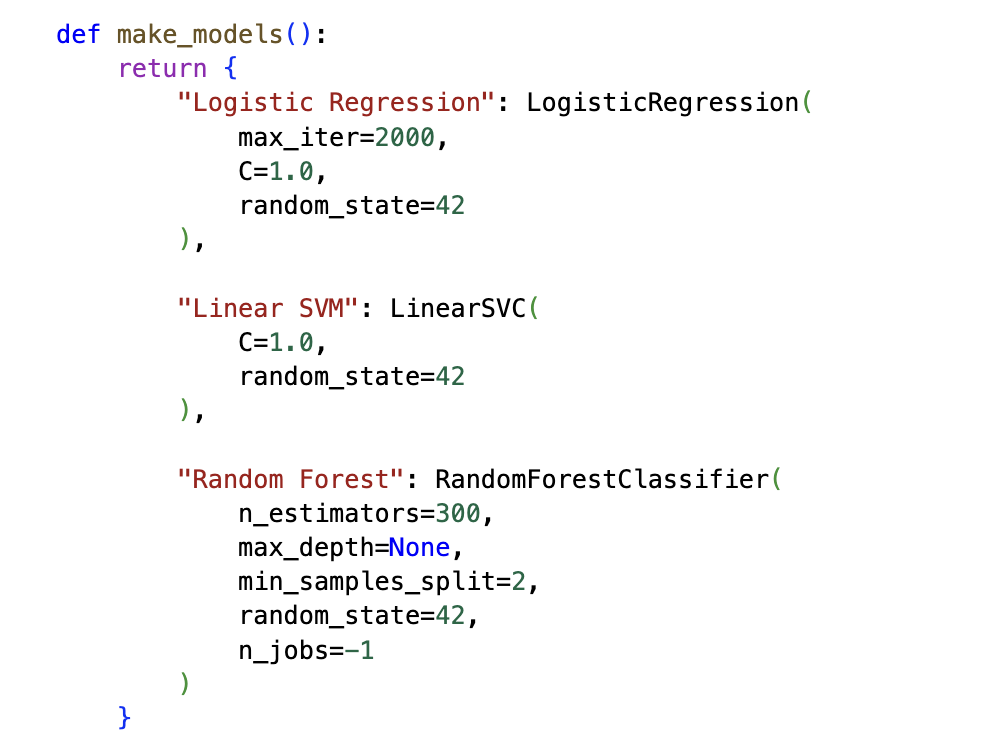
\includegraphics[width=0.78\textwidth]
    {figures/model_configuration.png}
    \caption{Configuration of Machine-Learning Models Used for Training}
    \label{fig:model_configuration}
\end{figure}

For each feature configuration, the classifiers are fitted using the
corresponding training feature matrix and training labels. The trained
models are then stored together with their model and feature-set names
for subsequent testing.

The implementation of the training process is shown in
Figure~\ref{fig:model_training}.

\begin{figure}[H]
    \centering
    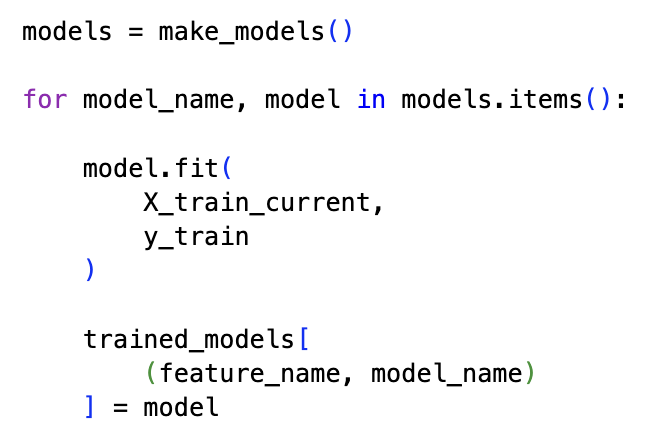
\includegraphics[width=0.52\textwidth]
    {figures/model_training.png}
    \caption{Training of Machine-Learning Models}
    \label{fig:model_training}
\end{figure}

\subsection{Testing (Performance Evaluation on Test Data)}

The twelve trained model--feature-set combinations are tested using
the 320 unseen test reviews. The same test samples are used for every
experiment to provide a consistent comparison between the models and
feature representations.

For each trained model, the \texttt{predict()} method is applied to
the corresponding test feature matrix to generate predicted class
labels. Logistic Regression and Random Forest use
\texttt{predict\_proba()} to obtain probability scores, while Linear
SVM uses \texttt{decision\_function()} because \texttt{LinearSVC}
does not directly provide class probabilities.

The implementation used to generate predictions and scores is shown
in Figure~\ref{fig:model_testing}.

\begin{figure}[H]
    \centering
    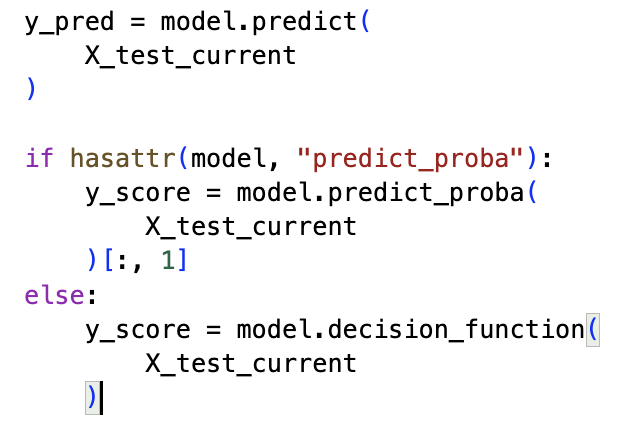
\includegraphics[width=0.52\textwidth]
    {figures/model_testing.png}
    \caption{Prediction of Class Labels and Scores on the Test Dataset}
    \label{fig:model_testing}
\end{figure}

The predicted labels and scores are retained for performance
evaluation using Accuracy, Precision, Recall, F1-score, ROC--AUC, and
the Confusion Matrix.

\newpage
% =========================================================
% CHAPTER 5
% RESULTS AND DISCUSSION
% =========================================================

\chapter{Results and Discussion}

This chapter presents and discusses the experimental results obtained
from the Fake Review Detection system. The evaluation was performed
using the unseen test dataset containing 320 reviews, consisting of
160 fake/deceptive reviews and 160 genuine/truthful reviews.

Three machine-learning classifiers---Logistic Regression, Linear SVM,
and Random Forest---were evaluated using four feature configurations:
TF-IDF, TF-IDF + Linguistic Features, TF-IDF + VADER Features, and
TF-IDF + Linguistic + VADER Features. This resulted in twelve
model--feature-set combinations.

The analysis focuses on the performance of the classifiers and the
contribution of linguistic and sentiment-based information beyond the
TF-IDF baseline. Accuracy, Precision, Recall, F1-score, ROC--AUC, and
the Confusion Matrix were used for evaluation.

% =========================================================
% 5.1 MODEL PERFORMANCE AND EVALUATION
% =========================================================

\section{Model Performance and Evaluation}

The twelve experimental configurations were evaluated using Accuracy,
Precision, Recall, F1-score, and ROC--AUC. These measures provide
different perspectives on the ability of the models to distinguish
fake reviews from genuine reviews.

Fake/deceptive reviews are represented by Label 1 and genuine/truthful
reviews by Label 0. Therefore, True Positive (TP) represents a fake
review correctly classified as fake, True Negative (TN) represents a
genuine review correctly classified as genuine, False Positive (FP)
represents a genuine review incorrectly classified as fake, and False
Negative (FN) represents a fake review incorrectly classified as
genuine.

\noindent\textbf{Accuracy}

Accuracy represents the overall proportion of correctly classified
reviews and is calculated as:

\begin{equation}
\text{Accuracy} =
\frac{\text{TP} + \text{TN}}
{\text{TP} + \text{TN} + \text{FP} + \text{FN}}
\end{equation}

\noindent\textbf{Precision}

Precision represents the proportion of reviews predicted as fake that
are actually fake:

\begin{equation}
\text{Precision} =
\frac{\text{TP}}
{\text{TP} + \text{FP}}
\end{equation}

\noindent\textbf{Recall}

Recall represents the proportion of actual fake reviews that are
correctly identified:

\begin{equation}
\text{Recall} =
\frac{\text{TP}}
{\text{TP} + \text{FN}}
\end{equation}

\noindent\textbf{F1-score}

F1-score represents the harmonic mean of Precision and Recall:

\begin{equation}
\text{F1-score} =
2 \times
\frac{\text{Precision} \times \text{Recall}}
{\text{Precision} + \text{Recall}}
\end{equation}

\noindent\textbf{ROC--AUC}

ROC--AUC measures the ability of a classifier to discriminate between
fake and genuine reviews across different classification thresholds.
For Logistic Regression and Random Forest, probability scores were
used, whereas the scores generated by the
\texttt{decision\_function()} were used for Linear SVM.

Figure~\ref{fig:model_comparison} presents the performance obtained
from all twelve model--feature-set combinations.

\begin{figure}[H]
    \centering
    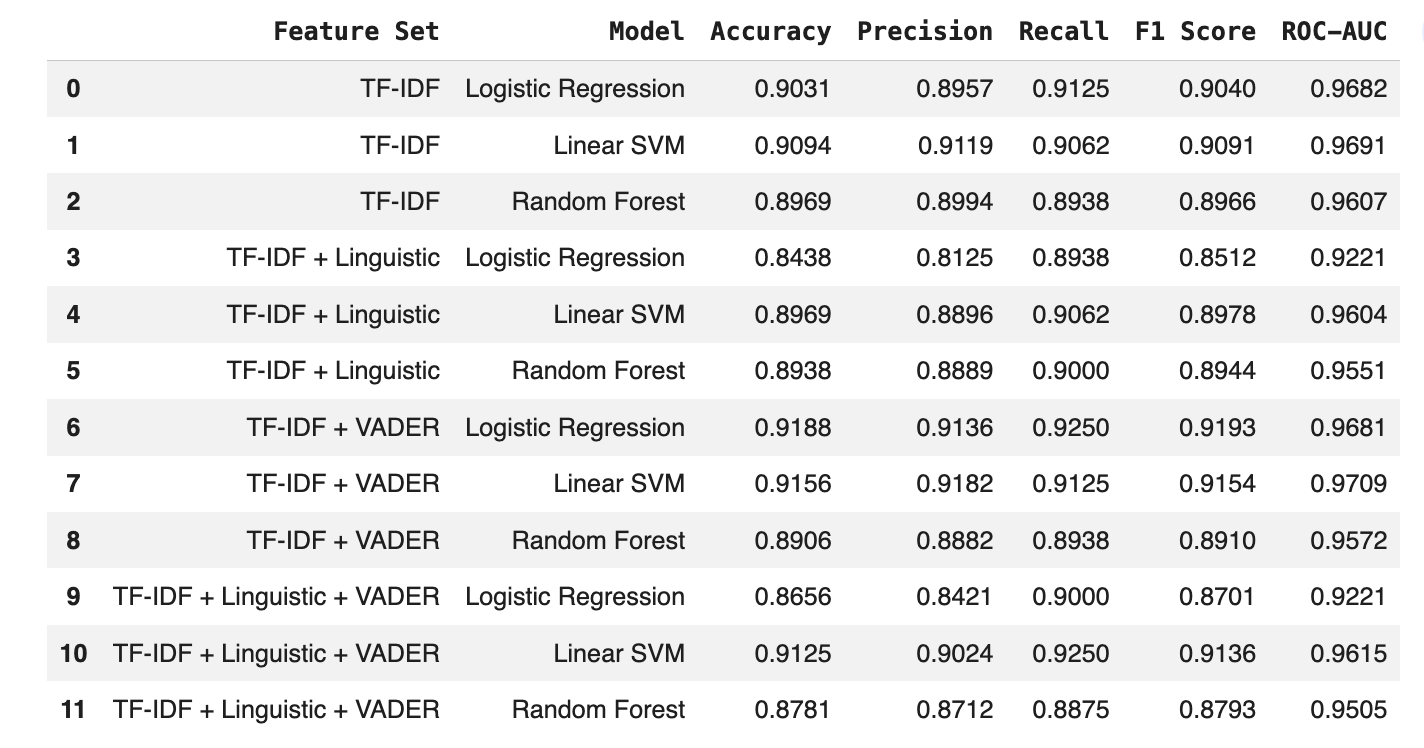
\includegraphics[width=\textwidth]
    {figures/model_comparison.png}
    \caption{Performance Comparison of Model--Feature-Set Combinations}
    \label{fig:model_comparison}
\end{figure}

TF-IDF alone provided a strong baseline for fake-review
classification. Logistic Regression achieved an accuracy of 90.31\%,
Linear SVM achieved 90.94\%, and Random Forest achieved 89.69\%.

Among all twelve experimental configurations, Logistic Regression with
TF-IDF + VADER achieved the highest Accuracy of 91.88\% and the
highest F1-score of 91.93\%. Linear SVM with TF-IDF + VADER achieved
the highest Precision of 91.82\% and the highest ROC--AUC of 97.09\%.
The highest Recall of 92.50\% was obtained by Logistic Regression with
TF-IDF + VADER and Linear SVM with TF-IDF + Linguistic + VADER.

These results indicate that the different model--feature combinations
provide different advantages. Therefore, the performance of the models
is analysed using multiple evaluation measures rather than accuracy
alone.

% =========================================================
% 5.2 FEATURE CONTRIBUTION ANALYSIS
% =========================================================

\section{Feature Contribution Analysis}

The feature-contribution analysis examines whether linguistic and
sentiment-based information provides additional predictive value
beyond the TF-IDF textual representation.

\noindent\textbf{TF-IDF Baseline}

TF-IDF alone produced strong classification results for all three
models. Logistic Regression achieved 90.31\% accuracy, Linear SVM
achieved 90.94\%, and Random Forest achieved 89.69\%. This indicates
that lexical and phrase-level information within the review text
contains substantial predictive information.

\vspace{0.3cm}
\noindent\textbf{Contribution of Linguistic Features}

The contribution of the six linguistic features was examined by
comparing TF-IDF with TF-IDF + Linguistic Features.

For Logistic Regression, accuracy decreased from 90.31\% to 84.38\%,
a reduction of 5.93 percentage points. Linear SVM decreased from
90.94\% to 89.69\%, a reduction of 1.25 percentage points, while
Random Forest decreased from 89.69\% to 89.38\%, a reduction of
0.31 percentage points.

Therefore, the selected linguistic features did not improve
classification accuracy over the TF-IDF baseline for any of the
three classifiers under the current experimental setup. This does not
indicate that linguistic information is generally unhelpful; rather,
the six selected features did not provide additional predictive value
in the present experiment.
Although the reviewed literature demonstrates that linguistic
features can improve fake review detection, the present
experiment produced different results. This variation may
be associated with differences in dataset characteristics
and feature representations. Previous studies examined
different review datasets and broader combinations of
linguistic, semantic, and behavioural features, whereas
the present study used six structural linguistic features
extracted from hotel reviews.

Additionally, TF-IDF already captures important textual
patterns, and the selected linguistic features may not
have provided sufficient complementary information to
improve classification performance. The observed decrease
in accuracy does not establish that linguistic features
are ineffective in general. Instead, it highlights that
the usefulness of additional features depends on the
dataset, selected characteristics, and classification
algorithm.

\vspace{0.3cm}
\noindent\textbf{Contribution of VADER Sentiment Features}

The contribution of sentiment information was examined by comparing
TF-IDF with TF-IDF + VADER Features.

For Logistic Regression, accuracy increased from 90.31\% to 91.88\%.
Precision increased from 89.57\% to 91.36\%, Recall increased from
91.25\% to 92.50\%, and F1-score increased from 90.40\% to 91.93\%.
ROC--AUC remained almost unchanged, changing from 96.82\% to 96.81\%.

For Linear SVM, accuracy increased from 90.94\% to 91.56\%.
Precision increased from 91.19\% to 91.82\%, Recall increased from
90.62\% to 91.25\%, F1-score increased from 90.91\% to 91.54\%, and
ROC--AUC increased from 96.91\% to 97.09\%.

Random Forest showed a different pattern. Its accuracy decreased from
89.69\% to 89.06\%, while its F1-score decreased from 89.66\% to
89.10\%.

These results indicate that the contribution of VADER sentiment
information is model-dependent. It provided additional predictive
value for Logistic Regression and Linear SVM, while the same
improvement was not observed for Random Forest.

\vspace{0.3cm}
\noindent\textbf{Combined Feature Contribution}

The complete feature representation combines TF-IDF, linguistic
features, and VADER sentiment features.

Using this representation, Logistic Regression achieved 86.56\%
accuracy, Linear SVM achieved 91.25\%, and Random Forest achieved
87.81\%.

Compared with TF-IDF + VADER, adding the linguistic features reduced
accuracy for all three classifiers. Therefore, combining all available
features did not produce the highest classification performance.

This demonstrates that increasing the number of features does not
necessarily improve classification performance. The usefulness of
additional features depends on the information they provide and how
the learning algorithm uses that information.

\vspace{0.3cm}
\noindent\textbf{Accuracy Comparison}

Figure~\ref{fig:accuracy_comparison} presents the accuracy obtained by
the three classifiers across the four feature configurations.

\begin{figure}[H]
    \centering
    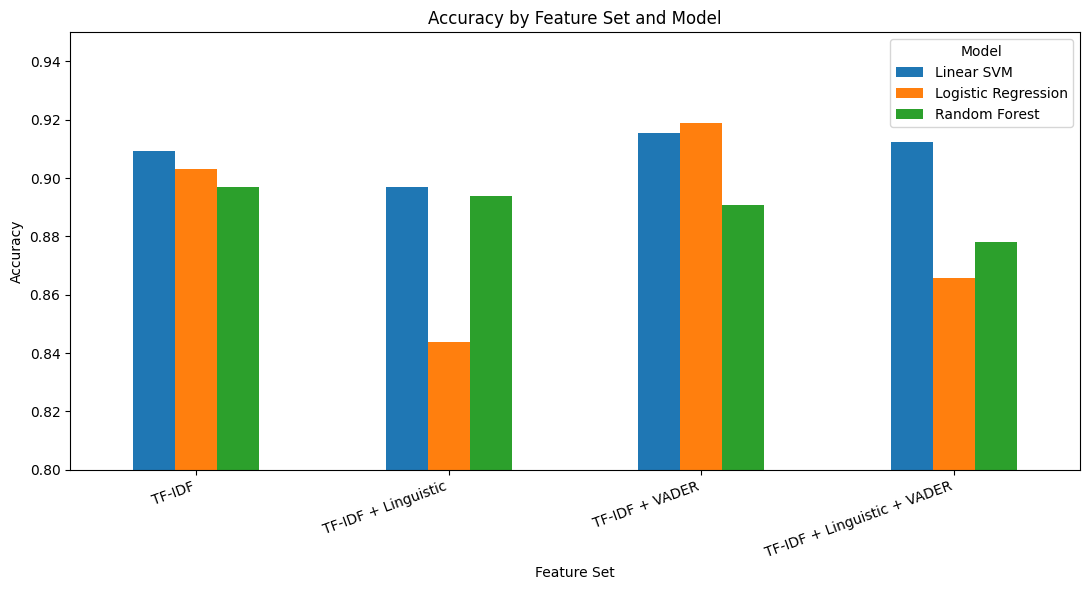
\includegraphics[width=0.95\textwidth]
    {figures/comparison.png}
    \caption{Accuracy Comparison Across Feature Sets and Classification Models}
    \label{fig:accuracy_comparison}
\end{figure}

The accuracy comparison clearly shows that TF-IDF provides a strong
baseline. The addition of VADER features improves Logistic Regression
and Linear SVM, whereas the selected linguistic features do not
produce an accuracy improvement over the baseline.

\vspace{0.3cm}
\noindent\textbf{F1-Score Comparison}

Figure~\ref{fig:f1_comparison} presents the F1-score obtained across
the feature configurations.

\begin{figure}[H]
    \centering
    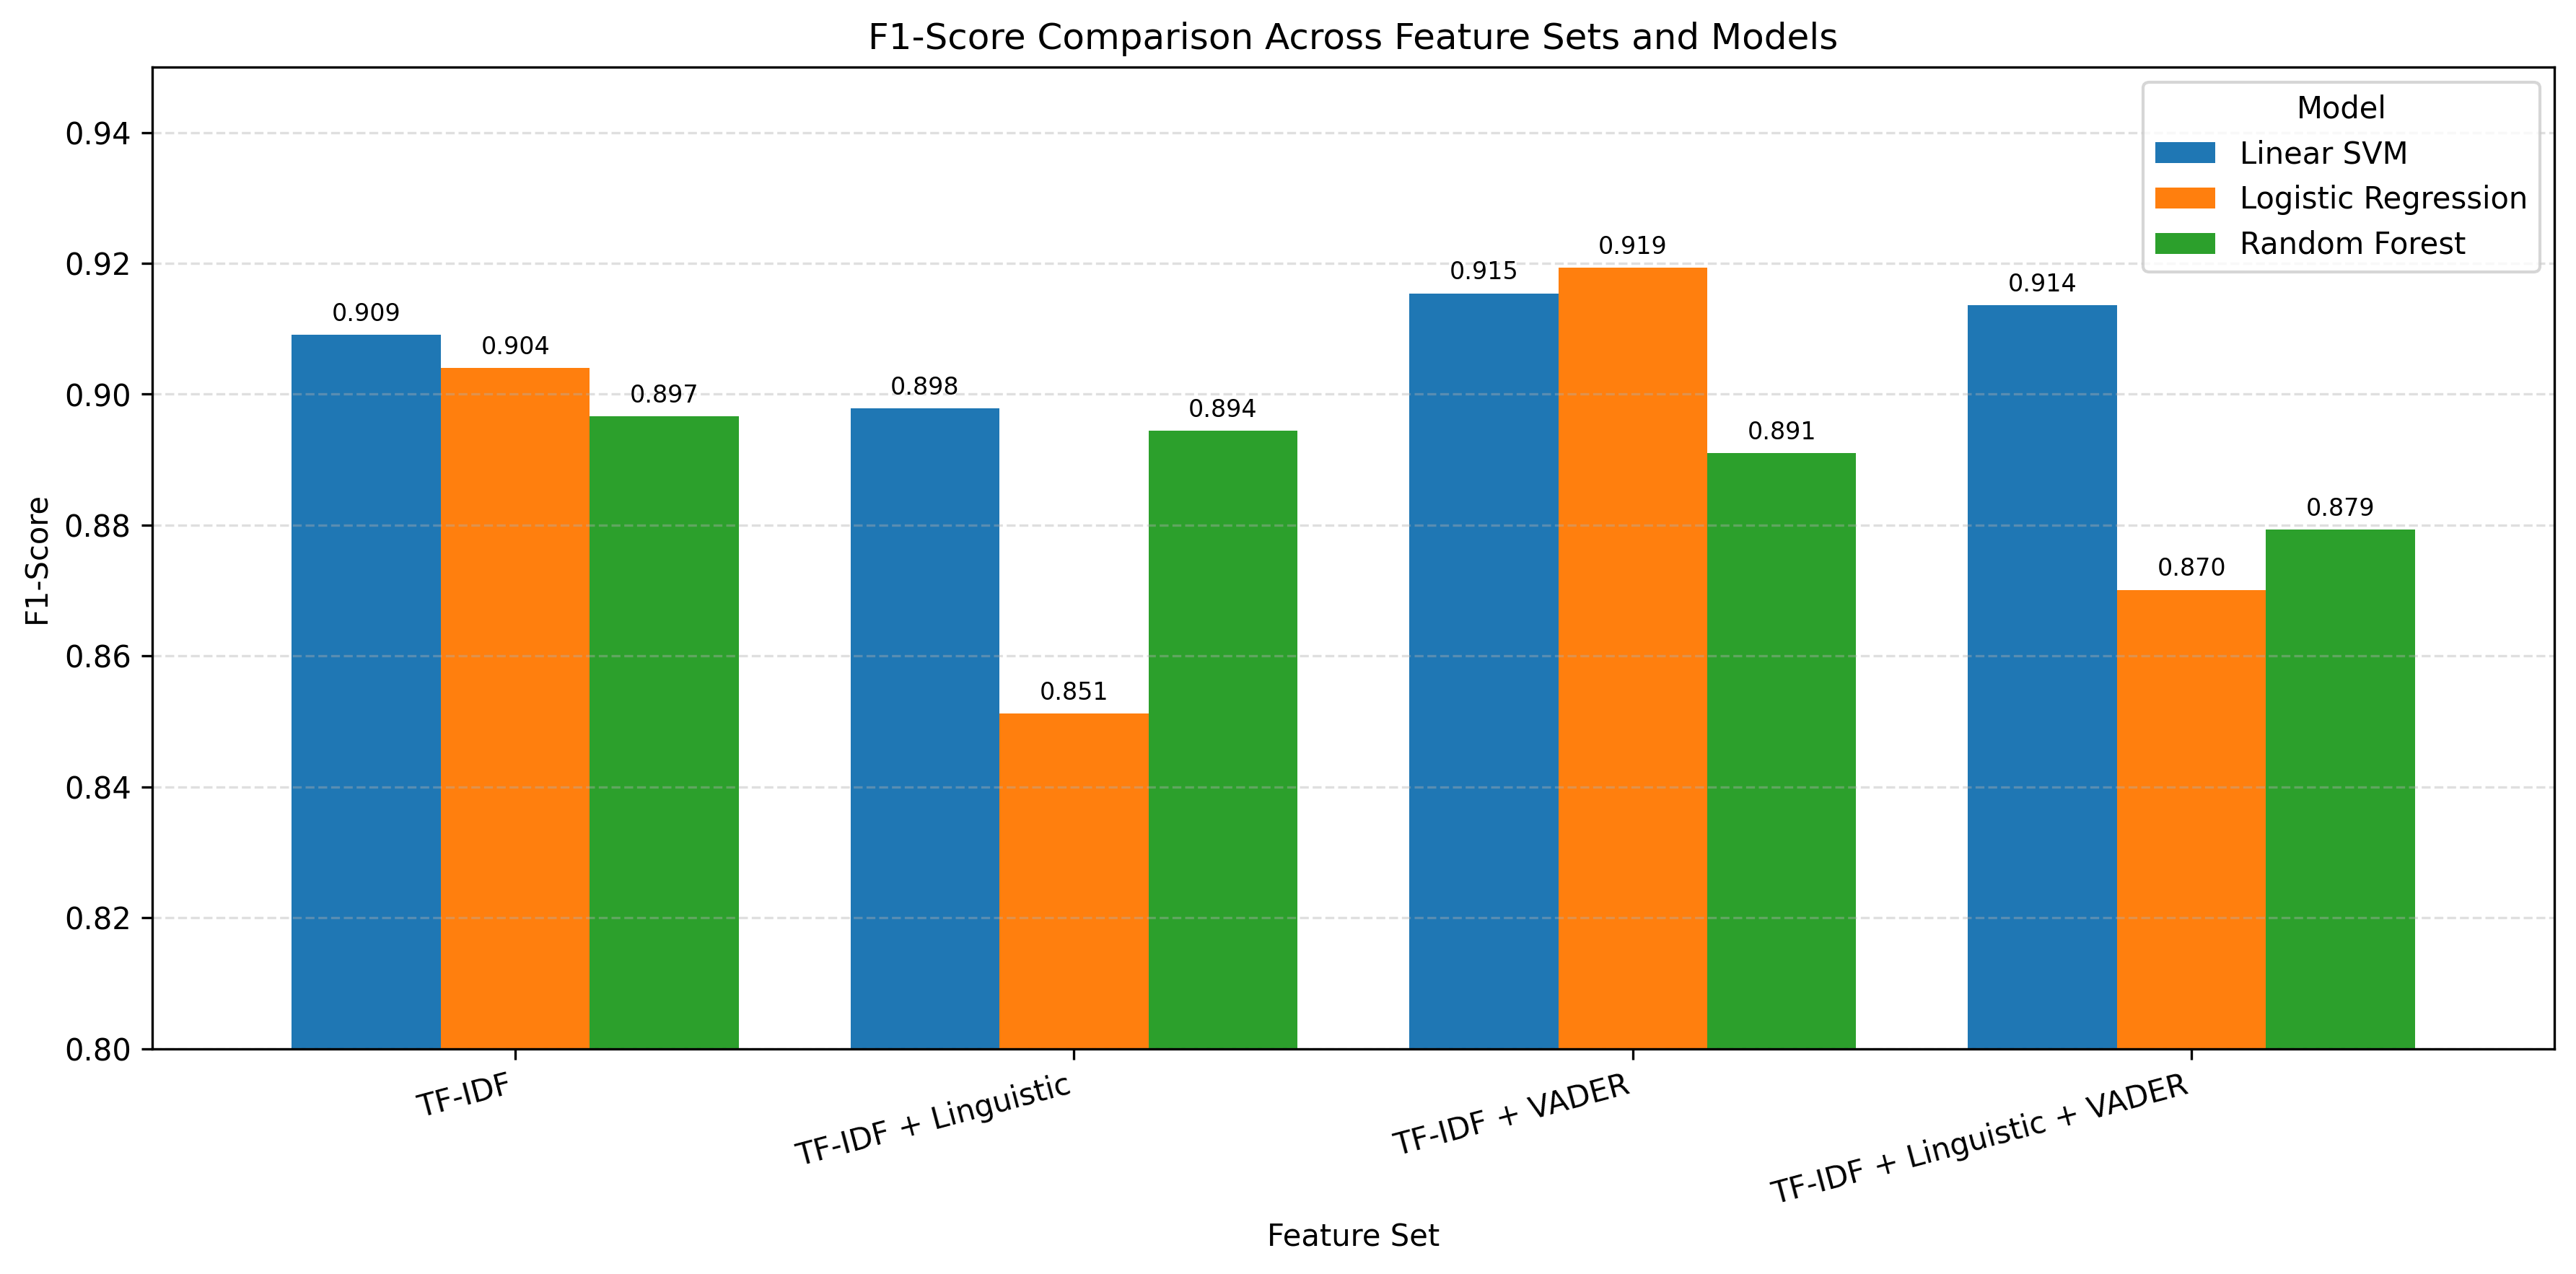
\includegraphics[width=0.95\textwidth]
    {figures/f1_comparison.png}
    \caption{F1-score Comparison Across Feature Sets and Classification Models}
    \label{fig:f1_comparison}
\end{figure}

The F1-score comparison follows a similar pattern to the accuracy
results. Logistic Regression with TF-IDF + VADER achieved the
highest F1-score of 91.93\%.

% =========================================================
% 5.3 ROC-AUC ANALYSIS
% =========================================================

\section{ROC--AUC Analysis}

ROC--AUC was used to evaluate the ability of the classifiers to
discriminate between fake/deceptive and genuine/truthful reviews
across different classification thresholds.

The Receiver Operating Characteristic (ROC) curve represents the
relationship between the True Positive Rate and False Positive Rate.
A larger area under the ROC curve indicates stronger discrimination
between the two classes.

Figure~\ref{fig:roc_comparison} presents the ROC curves obtained using
the TF-IDF + VADER feature configuration for the three classifiers.

\begin{figure}[H]
    \centering
    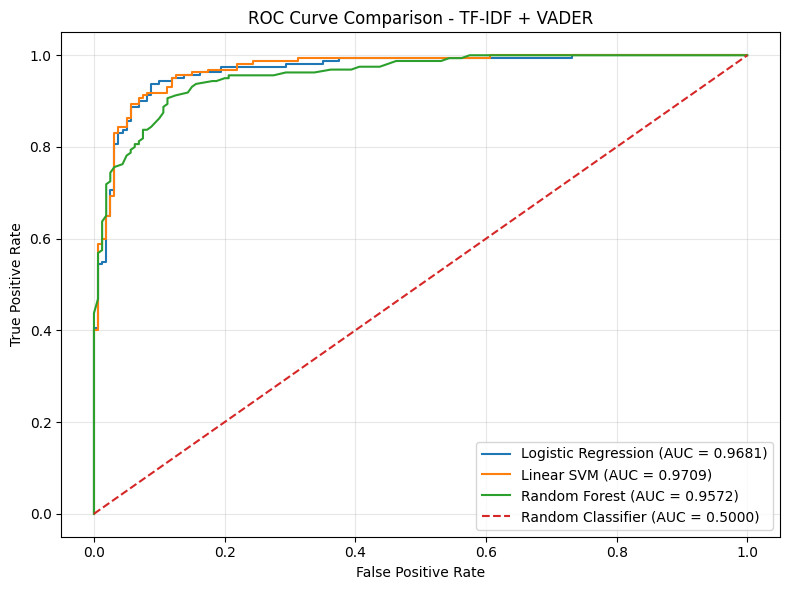
\includegraphics[width=0.80\textwidth]
    {figures/roc-auc.png}
    \caption{ROC Curve Comparison for TF-IDF + VADER Models}
    \label{fig:roc_comparison}
\end{figure}

For the TF-IDF + VADER configuration, Linear SVM achieved the highest
ROC--AUC value of 0.9709, followed by Logistic Regression with 0.9681
and Random Forest with 0.9572.

Although Linear SVM achieved the highest ROC--AUC, Logistic Regression
with TF-IDF + VADER achieved the highest Accuracy and F1-score.
Therefore, multiple evaluation measures were considered when analysing
the overall model performance.

% =========================================================
% 5.4 CONFUSION MATRIX ANALYSIS
% =========================================================

\section{Confusion Matrix Analysis}

Logistic Regression with TF-IDF + VADER was selected for detailed
analysis because it achieved the highest Accuracy and F1-score among
the twelve evaluated configurations.

The confusion matrix provides a detailed representation of correct and
incorrect classifications. True Positive represents a fake review
correctly classified as fake, while True Negative represents a genuine
review correctly classified as genuine. False Positive represents a
genuine review incorrectly classified as fake, whereas False Negative
represents a fake review incorrectly classified as genuine.

Figure~\ref{fig:confusion_matrix} shows the confusion matrix obtained
for Logistic Regression with TF-IDF + VADER.

\begin{figure}[H]
    \centering
    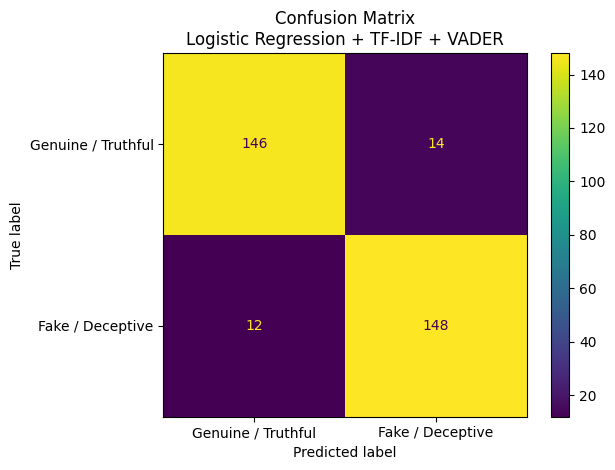
\includegraphics[width=0.65\textwidth]
    {figures/con.png}
    \caption{Confusion Matrix of Logistic Regression with TF-IDF + VADER}
    \label{fig:confusion_matrix}
\end{figure}

The diagonal elements of the confusion matrix represent correctly
classified reviews, while the off-diagonal elements represent
classification errors.

Table~\ref{tab:selected_model_metrics} summarizes the evaluation
results obtained by the selected configuration.

\begin{table}[H]
\centering

\begin{tabular}{|l|c|}
\hline
\textbf{Evaluation Metric} & \textbf{Result} \\ \hline
Accuracy & 91.88\% \\ \hline
Precision & 91.36\% \\ \hline
Recall & 92.50\% \\ \hline
F1-score & 91.93\% \\ \hline
ROC--AUC & 96.81\% \\ \hline
\end{tabular}
\caption{Performance of Logistic Regression with TF-IDF + VADER}
\label{tab:selected_model_metrics}
\end{table}

The Accuracy of 91.88\% indicates that a high proportion of the test
reviews were correctly classified. Precision of 91.36\% indicates
that most reviews predicted as fake were actually fake, while Recall
of 92.50\% indicates that the model identified a high proportion of
the actual fake reviews.

The F1-score of 91.93\% demonstrates a strong balance between
Precision and Recall. The ROC--AUC value of 96.81\% further indicates
strong discrimination between fake and genuine reviews.

% =========================================================
% 5.5 PREDICTION ON UNSEEN REVIEWS
% =========================================================

\section{Prediction and Testing on Unseen Reviews}

To examine the performance of the developed Fake Review
Detection System on previously unseen data, an external
labelled dataset of hotel reviews without overlap with
the training corpus was considered.

To evaluate the system under a balanced test configuration
comparable to the training class distribution, a balanced
evaluation dataset of 500 reviews was created through
stratified random sampling. The evaluation set contained
an equal distribution of 250 Fake/Deceptive reviews
and 250 Genuine/Truthful reviews.

The 500 unseen reviews were provided to the already-trained
Logistic Regression model without retraining or modifying
the existing prediction pipeline. Each review was processed
using the same preprocessing and feature extraction procedures
applied during model development. The cleaned review text
was transformed using the fitted TF-IDF vectorizer, while
VADER sentiment features were extracted from the original
review text and standardized using the fitted scaler.

The resulting TF-IDF and VADER features were combined
and supplied to the trained Logistic Regression
classifier. The predicted labels were compared with
the actual ground-truth labels to determine whether each
review was correctly classified.

Out of the 500 unseen reviews tested, the model correctly
classified 452 reviews, while 48 reviews were
incorrectly classified. These results indicate that
the model maintained consistent classification ability
on independent, unseen review data.

\begin{table}[H]
\centering

\begin{tabular}{|l|c|}
\hline
\textbf{Description} & \textbf{Number of Reviews} \\ \hline
Total Balanced Reviews Tested & 500 \\ \hline
Fake / Deceptive Reviews Tested & 250 \\ \hline
Genuine / Truthful Reviews Tested & 250 \\ \hline
Correctly Classified Reviews & 452 \\ \hline
Incorrectly Classified Reviews & 48 \\ \hline
\end{tabular}
\caption{Summary of External Dataset Testing}
\label{tab:external_testing_summary}
\end{table}

\subsection{Example Review Predictions}

To demonstrate the practical operation of the
prediction system, four reviews from the external
dataset were individually entered into the
Streamlit web application.

The system processed each review and displayed
the predicted class together with the estimated
fake and genuine probabilities.

The following examples illustrate the prediction
results obtained through the developed application.

\vspace{0.3cm}
\noindent\textbf{Review 1}

\begin{quote}
We booked a room at the Hilton Chicago for two nights to stay the
weekend but upon arrival our reservation could not be found. I even
provided the hotel with our confirmation number but it still wasn't
available! Fortunately another reservation had not shown up so there
was space available for us. Once we settled into our room for the
night (after a long flight), there was a bad odor coming from the
bathroom. Apparently the cleaning solution they used was tainted and
they had to re-clean it after our arrival. Needless to say, with both
of these poor experiences in just one night, I will be hesitant to
EVER stay in this hotel again, let alone any other Hilton around.
Please consider someplace else before the Hilton Chicago!
\end{quote}

\noindent
\textbf{Predicted Class:} Fake / Deceptive Review \\
\textbf{Fake Probability:} 72.69\% \\
\textbf{Genuine Probability:} 27.31\%

\vspace{0.5cm}
\noindent\textbf{Review 2}

\begin{quote}
Excellent location, feels like a boutique hotel. Right next to Neiman
Marcus (V.expensive dept store) and 2 mins walk to John Hancock tower.
As most American medium to high end hotels service was excellent from
the bellhop to reception. Upgrade to a suite if you are staying longer
than a couple of days as walking around the windy city can be tiring
and a suite feels like a small apartment. The pub in the basement is
good for a sandwich and a Beer. They will be refurbing so take
adavantage of lower rates now as I feel they will be going for very
high end clients after the remodelling.
\end{quote}

\noindent
\textbf{Predicted Class:} Genuine / Truthful Review \\
\textbf{Fake Probability:} 27.51\% \\
\textbf{Genuine Probability:} 72.49\%

\newpage

\vspace{0.5cm}
\noindent\textbf{Review 3}

\begin{quote}
Extremely disappointed in our stay. This hotel did not look like what
pictures portrayed online. I booked online thinking what a perfect
place this was going to be, only to arrive and have a room without a
view even though that is what was paid for. The room smelled musty and
not clean. Garbage was not changed from prior person. Found small ants
in bathroom near shower. Called to complain and someone came up 2
hours later and used bug spray. Overall this hotel is in a great
location, but we would never visit again. Staff was not overly
friendly or helpful and the room was not as all as it seemed online.
\end{quote}

\noindent
\textbf{Predicted Class:} Fake / Deceptive Review \\
\textbf{Fake Probability:} 53.38\% \\
\textbf{Genuine Probability:} 46.62\%

\vspace{0.5cm}
\noindent\textbf{Review 4}

\begin{quote}
My husband \& I stayed at the Fitzpatrick in early June 2004 for my
birthday-great hotel! Location provides easy walking to Navy Pier,
Marshall Field, Michigan Avenue \& John Hancock. Room seemed spacious
even though its only about 300 sq ft. Lots of room in bathroom;
comfortable bed; very quiet, upscale hotel. We would definitely stay
here again!
\end{quote}

\noindent
\textbf{Predicted Class:} Genuine / Truthful Review \\
\textbf{Fake Probability:} 23.69\% \\
\textbf{Genuine Probability:} 76.31\%

\vspace{0.5cm}
\noindent\textbf{Prediction Summary}

\begin{table}[H]
\centering

\resizebox{\textwidth}{!}{
\begin{tabular}{|c|>{\raggedright\arraybackslash}p{7cm}|c|c|c|}
\hline

\textbf{No.} &
\textbf{Review Summary} &
\textbf{Predicted Class} &
\textbf{Fake Probability} &
\textbf{Genuine Probability} \\ \hline

1 &
Reservation difficulties, unpleasant bathroom odor,
and negative hotel experience &
Fake / Deceptive &
72.69\% &
27.31\% \\ \hline

2 &
Positive description of hotel location, service,
room upgrade, and facilities &
Genuine / Truthful &
27.51\% &
72.49\% \\ \hline

3 &
Negative experience involving room condition,
cleanliness, insects, and poor service &
Fake / Deceptive &
53.38\% &
46.62\% \\ \hline

4 &
Positive experience describing hotel location,
room facilities, and willingness to return &
Genuine / Truthful &
23.69\% &
76.31\% \\ \hline

\end{tabular}
}
\caption{Prediction Results for Selected External Reviews}
\label{tab:unseen_predictions}
\end{table}

\subsection{Inference from External Testing}

The external testing demonstrated that the
trained Logistic Regression model was able to
classify a substantial number of previously
unseen hotel reviews without additional training.

Among the 500 balanced unseen reviews tested,
452 were classified correctly and 48 were
classified incorrectly. This indicates that
the model was able to recognize patterns
associated with deceptive and truthful reviews
in a separate, unseen dataset.

The four selected examples further demonstrate
the practical functionality of the Streamlit
application. Two reviews were predicted as
Fake/Deceptive and two were predicted as
Genuine/Truthful.

The estimated fake probabilities varied across
the examples, reflecting differences in the
model's confidence. The third review produced
a fake probability of 53.38\%, indicating
a prediction close to the classification
threshold.

Since these examples were selected from the
labelled external dataset, their predictions
can be compared with the corresponding actual
labels to determine individual correctness.

The results also show that the system does not
classify every review correctly. Differences
in writing style, vocabulary, and sentiment
expression may influence the predictions.

Overall, the external testing supports the
practical applicability of the developed
system for identifying potentially deceptive
hotel reviews. However, the predicted
classification should be treated as a
machine learning assessment rather than
definitive proof of review authenticity.

% =========================================================
% DISCUSSION OF FINDINGS
% =========================================================

\section{Discussion of Findings}

The experimental results provide several observations regarding the
use of review-text information for fake-review detection.

First, TF-IDF alone produced strong classification performance across
all three algorithms, with accuracies ranging from 89.69\% to 90.94\%.
This indicates that lexical and phrase-level information within review
text contains substantial predictive information.

Second, the selected linguistic features did not improve
classification accuracy when added to TF-IDF. The reduction was
largest for Logistic Regression and smaller for Linear SVM and Random
Forest, indicating that these features did not provide additional
predictive value under the present experimental setup.

Third, VADER sentiment features improved the two linear classifiers.
Logistic Regression improved from 90.31\% to 91.88\% accuracy, while
Linear SVM improved from 90.94\% to 91.56\%. Random Forest did not
show the same improvement, indicating that the contribution of
sentiment information depends on the learning algorithm.

The complete TF-IDF + Linguistic + VADER representation did not
produce the strongest overall performance, showing that increasing
the number of features does not necessarily improve classification.

Among the evaluated configurations, Logistic Regression with
TF-IDF + VADER achieved the highest Accuracy of 91.88\% and F1-score
of 91.93\%, while Linear SVM with TF-IDF + VADER achieved the highest
Precision of 91.82\% and ROC--AUC of 97.09\%.

Logistic Regression with TF-IDF + VADER was selected for the final
prediction pipeline based on its Accuracy and F1-score performance and
its ability to provide probability estimates through
\texttt{predict\_proba()}.

Overall, TF-IDF provided a strong textual baseline, while VADER
sentiment information provided additional value for Logistic
Regression and Linear SVM. The selected linguistic features did not
improve performance over the TF-IDF baseline in this experiment.

\newpage

\chapter{Model Deployment}

The proposed Fake Review Detection system is deployed using a
Streamlit-based web application that integrates the trained machine
learning model for real-time classification of hotel reviews.
The selected Logistic Regression model, trained using TF-IDF
and VADER sentiment features, is stored in serialized form
(\texttt{logistic\_regression\_model.pkl}) and loaded at runtime
using Joblib. The fitted TF-IDF vectorizer and VADER scaler
are also saved and loaded to ensure consistency between
the training and deployment environments.

When a user accesses the application, a text input interface
allows them to enter a hotel review for analysis. The submitted
review undergoes input validation, followed by text preprocessing
operations such as lowercase conversion, removal of HTML tags,
URLs, numbers and punctuation, tokenization, stop-word removal,
and lemmatization. The cleaned text is transformed into numerical
features using the saved TF-IDF vectorizer. Simultaneously,
VADER sentiment analysis is performed on the original review
to extract positive, negative, neutral, and compound sentiment
scores. These sentiment features are standardized using the
saved VADER scaler.

Once feature extraction is complete, the TF-IDF and scaled
VADER features are combined into a single feature vector
and passed to the trained Logistic Regression classifier.
The model classifies the review as either Fake (Deceptive)
or Genuine (Truthful) and generates the corresponding
prediction probabilities. The classification result is
displayed through the Streamlit interface in a clear
and user-friendly manner.

To improve transparency, the application also provides
a detailed explanation of the prediction process.
This includes the preprocessed review text, important
TF-IDF terms, extracted VADER sentiment scores, and
the contributions of individual features to the
Logistic Regression decision score. The application
also incorporates input validation and error-handling
mechanisms to manage empty, insufficient, or
unrecognized review inputs and prevent invalid
submissions from proceeding to classification.

\section{Model Implementation and User Interface Design}

The deployed Fake Review Detection system provides an interactive
web interface through which users can submit hotel reviews and
obtain classification results. The application also presents the
main processing stages involved in generating the prediction,
improving the transparency and interpretability of the proposed
system. The following screenshots illustrate the user interface
and the prediction explanation provided by the deployed application.

\begin{figure}[htbp]
    \centering
    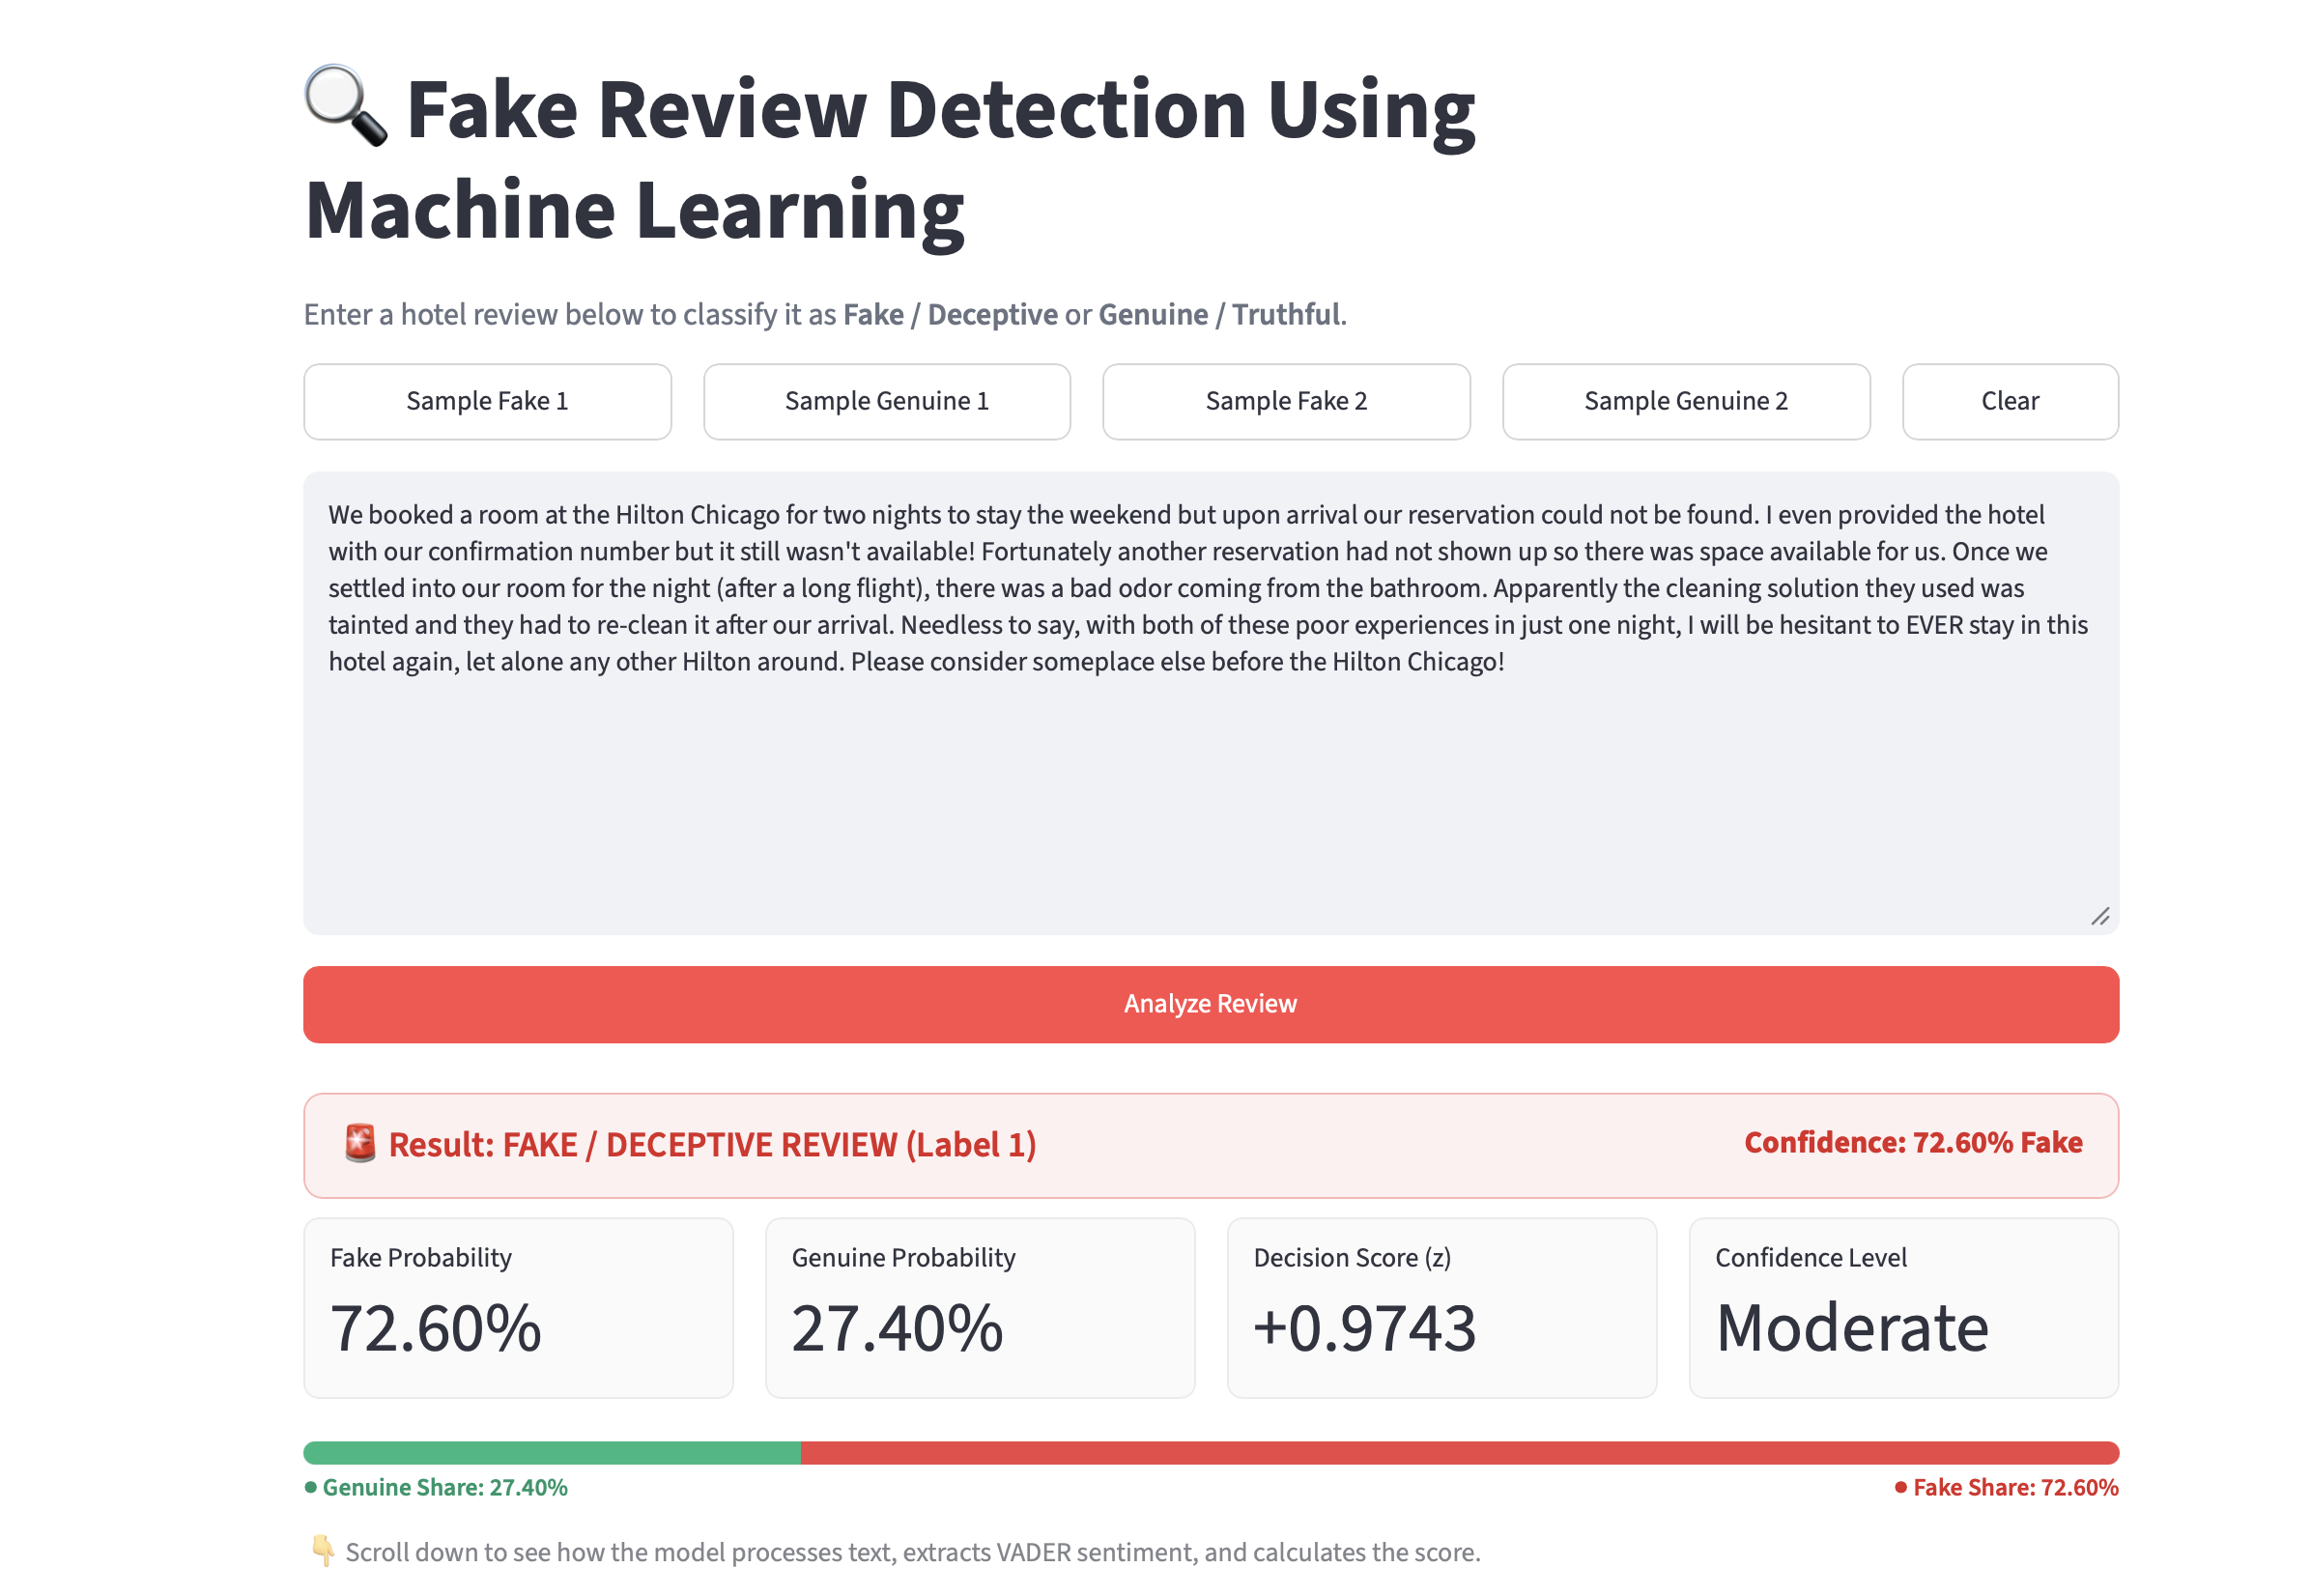
\includegraphics[width=\textwidth]{figures/deployment_result.png}
    \caption{Hotel review classification result and prediction probabilities.}
    \label{fig:deployment_result}
\end{figure}

Figure~\ref{fig:deployment_result} shows the main interface of the
deployed application. The user can enter a hotel review and click
the \textit{Analyze Review} button to obtain a prediction. The
application displays the predicted class as either Fake/Deceptive
or Genuine/Truthful, along with the corresponding prediction
probabilities.

\begin{figure}[htbp]
    \centering
    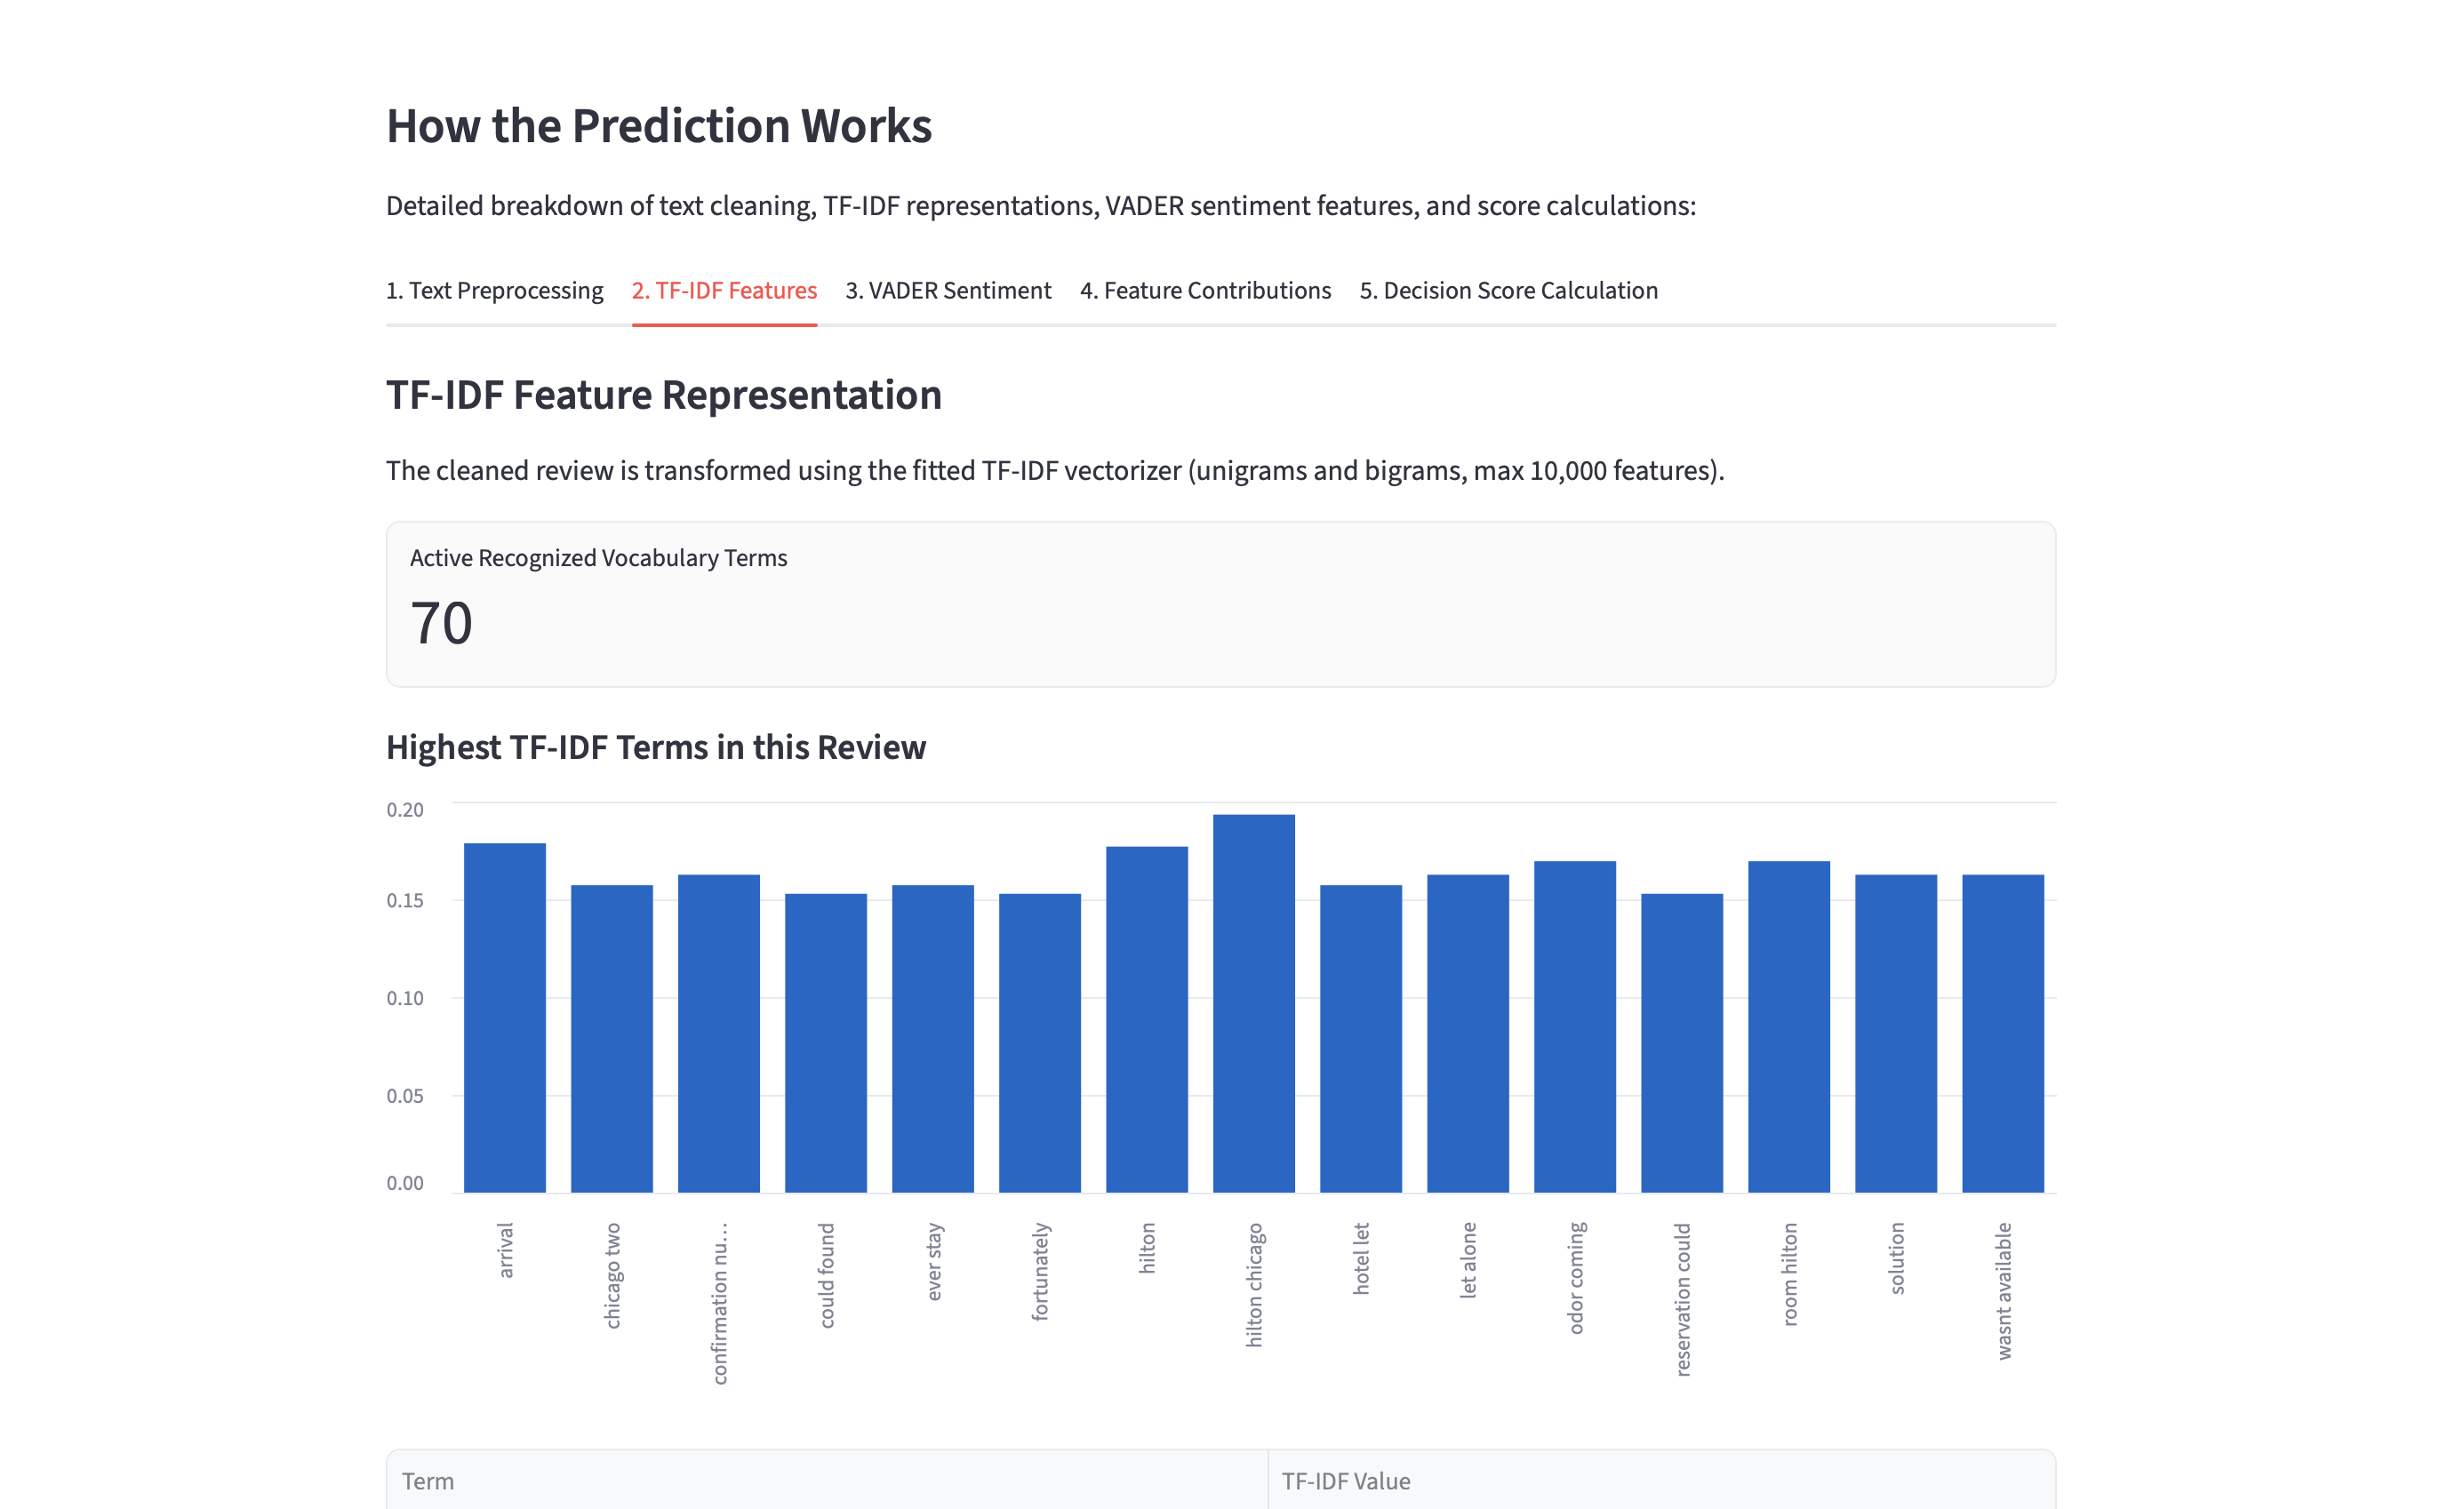
\includegraphics[width=\textwidth]{figures/prediction_explanation.png}
    \caption{Explanation of the prediction process and
    Logistic Regression decision score.}
    \label{fig:prediction_explanation}
\end{figure}

\newpage

\chapter{Git History}

The Git repository for the Fake Review Detection Using Machine
Learning project contains the essential components required
for model development, evaluation, and web application
deployment. It includes Python scripts for data preprocessing,
feature extraction, model training, and evaluation, along with
the Streamlit application files used for the user interface.
The repository also maintains the serialized Logistic Regression
model, fitted TF-IDF vectorizer, and VADER scaler, which are
required for classifying hotel reviews.

Git and GitHub are used for version control, enabling the
tracking of code modifications, management of project updates,
and maintenance of different development stages. The
repository provides an organized structure for reviewing
the implementation, identifying errors, and making future
improvements. This version-controlled approach supports
project maintainability, reproducibility, and further
enhancement of the fake review detection system.

\noindent\textbf{GitHub Repository}

The project source code is maintained in a public GitHub
repository, which contains the files required for model
implementation and application deployment. The repository
includes the trained model components, dataset, application
code, and project documentation. GitHub is used to maintain
version history and track modifications made during development.

Figure~\ref{fig:github_repository} shows the GitHub repository
of the Fake Review Detection Using Machine Learning project,
including its directory structure.

\begin{figure}[htbp]
    \centering
    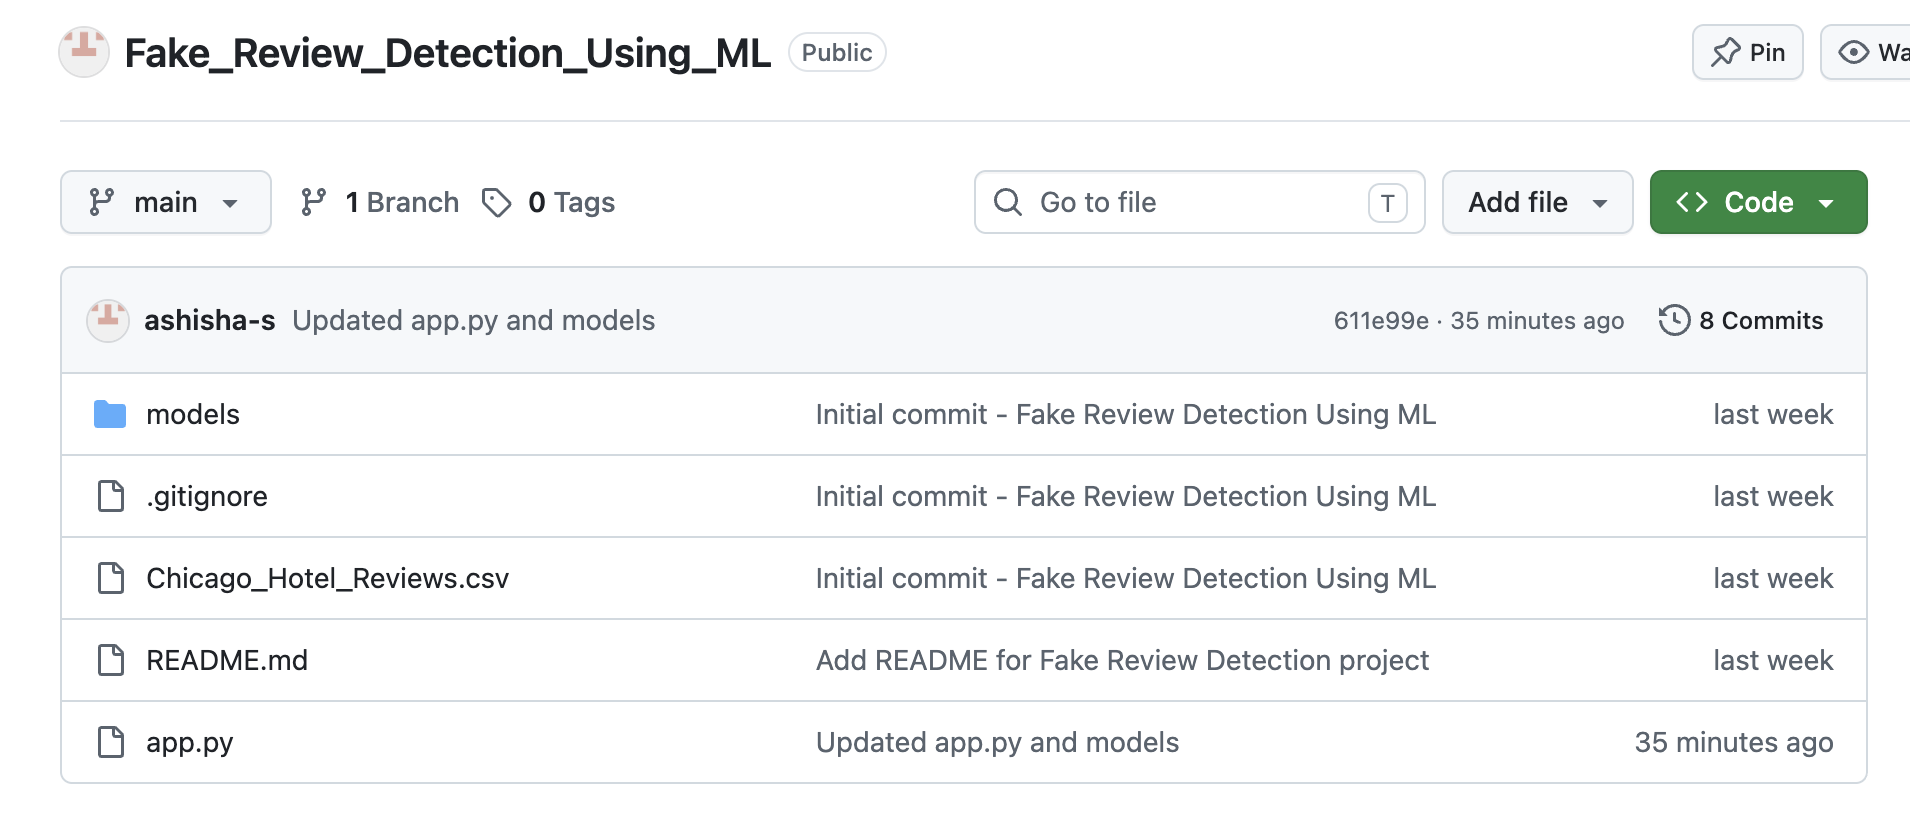
\includegraphics[width=\textwidth]{figures/github_repository.png}
    \caption{GitHub repository}
    \label{fig:github_repository}
\end{figure}

\newpage
\chapter{Conclusions}

In conclusion, the Fake Review Detection Using Machine Learning
project successfully achieved its objective of developing a
machine learning-based system for identifying deceptive and
genuine hotel reviews. The system was developed using the Ott
Deceptive Opinion Spam Corpus, containing 1,600 labelled hotel
reviews with an equal distribution of fake and genuine reviews.
Natural Language Processing techniques were applied for text
preprocessing, while TF-IDF, linguistic features, and VADER
sentiment analysis were used to extract relevant information
from the review text.

Three supervised machine learning algorithms, namely Logistic
Regression, Linear Support Vector Machine (SVM), and Random
Forest, were implemented and evaluated using four different
feature configurations. A total of twelve model--feature-set
combinations were compared using Accuracy, Precision, Recall,
F1-score, ROC--AUC, and Confusion Matrix. The experimental
results demonstrated that TF-IDF provided a strong baseline
for classification, while the addition of VADER sentiment
features improved the performance of Logistic Regression
and Linear SVM. However, the selected linguistic features
did not provide further improvement under the current
experimental setup.

Among the evaluated configurations, Logistic Regression
with TF-IDF and VADER sentiment features achieved the
highest Accuracy of 91.88\% and F1-score of 91.93\%.
The selected model also achieved a Precision of 91.36\%,
Recall of 92.50\%, and ROC--AUC of 96.81\%. Based on
its overall classification performance and ability to
generate probability estimates, Logistic Regression with
TF-IDF and VADER was selected for the final prediction
system.

The trained model was integrated into a Streamlit-based
web application to enable classification of user-submitted
hotel reviews. The application processes the review text,
extracts TF-IDF and VADER sentiment features, and generates
a prediction indicating whether the review is fake or genuine,
along with the corresponding classification probabilities.
The interface also provides information about the extracted
features and their contribution to the prediction, improving
the transparency and usability of the system.

Overall, the project demonstrates the effectiveness of
combining Natural Language Processing, sentiment analysis,
and classical machine learning techniques for detecting
deceptive online reviews. The experimental findings highlight
the importance of selecting suitable feature combinations
rather than simply increasing the number of features.
Although the system was developed and evaluated using
hotel reviews, it provides a foundation for future
enhancements involving larger datasets, additional review
domains, and more advanced classification techniques.

\newpage

\chapter{Future Work}

\begin{itemize}

    \item \textbf{Advanced Machine Learning Algorithms:}
    Future improvements can explore ensemble learning
    algorithms such as XGBoost and CatBoost, along with
    deep learning models such as LSTM and BERT, to improve
    classification accuracy and capture complex
    linguistic patterns.

    \item \textbf{Larger and Diverse Datasets:}
    The system can be trained on larger datasets containing
    reviews from e-commerce platforms, restaurants, and
    travel websites to improve generalization across
    different domains.

    \item \textbf{Advanced Feature Engineering:}
    Additional features such as semantic similarity,
    contextual embeddings, and readability scores can
    be incorporated to identify deceptive patterns
    more effectively.

    \item \textbf{Detection of AI-Generated Reviews:}
    The system can be extended to detect AI-generated
    deceptive reviews by incorporating appropriately
    labeled datasets containing machine-generated content.

    \item \textbf{Enhanced Explainability:}
    Explainable AI techniques such as SHAP and LIME
    can be integrated to provide more detailed
    interpretations of model predictions.

    \item \textbf{Multilingual Review Detection:}
    Future versions can support multiple languages
    through multilingual text preprocessing and
    language-specific feature extraction techniques.

    \item \textbf{Cloud Deployment and Platform Integration:}
    The Streamlit application can be deployed on cloud
    platforms and integrated with online review websites
    through APIs to enable scalable and automated
    review classification.

\end{itemize}

\newpage

\chapter{Appendix}

\section{Minimum Software Requirements}

\noindent
\textbf{Operating System:} Windows 10 / Linux / macOS

\noindent
\textbf{Python Version:} Python 3.10 or above

\vspace{0.3cm}

\noindent
\textbf{Required Libraries:}

\begin{itemize}
    \item Streamlit (for web application development)
    \item NumPy (for numerical operations)
    \item Pandas (for data manipulation and analysis)
    \item Scikit-learn (for feature extraction, model training,
    evaluation, and classification)
    \item NLTK (for text preprocessing, lemmatization,
    stop-word removal, and VADER sentiment analysis)
    \item SciPy (for sparse feature matrix operations)
    \item Joblib (for saving and loading trained models,
    vectorizers, and scalers)
    \item Matplotlib / Seaborn (for exploratory data analysis
    and visualization)
\end{itemize}

\noindent
\textbf{Development Tools:}

\begin{itemize}
    \item Google Colab / Jupyter Notebook (for data preprocessing,
    feature extraction, model training, and evaluation)
    \item Visual Studio Code (for Streamlit application development)
    \item Git / GitHub (for version control and repository management)
\end{itemize}

\noindent
\textbf{Browser:} Latest version of Google Chrome, Mozilla Firefox,
or Microsoft Edge for accessing the Streamlit web application.

\vspace{0.4cm}

\section{Minimum Hardware Requirements}

\begin{itemize}

    \item \textbf{Processor:}
    Dual-core 2.0 GHz processor or higher.
    A quad-core processor is recommended for faster
    data preprocessing and model training.

    \item \textbf{RAM:}
    Minimum 4 GB RAM, with 8 GB recommended
    for smooth execution of data analysis,
    machine learning operations, and the
    Streamlit web application.

    \item \textbf{Storage:}
    At least 2 GB of available disk space
    for the dataset, Python environment,
    trained model files, application code,
    and other project resources.

    \item \textbf{Display:}
    Standard display resolution of
    1366 $\times$ 768 pixels or higher.

    \item \textbf{Internet Connection:}
    An internet connection is required for:

    \begin{itemize}
        \item Installing Python libraries and dependencies.
        \item Downloading the hotel review dataset.
        \item Accessing Google Colab for model development
        and experimentation.
        \item Accessing GitHub for version control
        and repository management.
        \item Downloading required NLTK resources
        during initial setup.
    \end{itemize}

\end{itemize}

% ==========================================
% REFERENCES
% ==========================================

\newpage
\chapter{References}

\begin{enumerate}

    \item Khan A, Adnan M, Anwar S.
    Empowering Trust in Digital Platforms:
    Sentiment Analysis and Emotion AI for
    Fake Reviews Detection.
    IEEE Transactions on Computational Social Systems.
    2025. Early Access.
    Available from: https://doi.org/10.1109/TCSS.2025.3638615

    \item Abdulqader M, Namoun A, Alsaawy Y.
    Fake Online Reviews: A Unified Detection Model
    Using Deception Theories.
    IEEE Access. 2022;10:128622--128655.
    Available from: https://doi.org/10.1109/ACCESS.2022.3227631

    \item Janokar S, Joshi K, More K, Pawar P,
    Raikwar R, Singh T.
    Fake Review Detection System:
    A Machine Learning Approach with
    Linguistic and Semantic Analysis.
    In: Proceedings of the 2024 International
    Conference on Artificial Intelligence and
    Quantum Computation-Based Sensor Application
    (ICAIQSA). IEEE; 2024.
    Available from: https://doi.org/10.1109/ICAIQSA64000.2024.10882276

    \item Ott M, Choi Y, Cardie C, Hancock JT.
    Finding Deceptive Opinion Spam by Any
    Stretch of the Imagination.
    In: Proceedings of the 49th Annual Meeting
    of the Association for Computational Linguistics:
    Human Language Technologies. 2011.
    pp. 309--319.
    Available from: https://aclanthology.org/P11-1032/

\end{enumerate}
\end{document}